\documentclass[]{article}
\usepackage{lmodern}
\usepackage{amssymb,amsmath}
\usepackage{ifxetex,ifluatex}
\usepackage{fixltx2e} % provides \textsubscript
\ifnum 0\ifxetex 1\fi\ifluatex 1\fi=0 % if pdftex
  \usepackage[T1]{fontenc}
  \usepackage[utf8]{inputenc}
\else % if luatex or xelatex
  \ifxetex
    \usepackage{mathspec}
  \else
    \usepackage{fontspec}
  \fi
  \defaultfontfeatures{Ligatures=TeX,Scale=MatchLowercase}
\fi
% use upquote if available, for straight quotes in verbatim environments
\IfFileExists{upquote.sty}{\usepackage{upquote}}{}
% use microtype if available
\IfFileExists{microtype.sty}{%
\usepackage{microtype}
\UseMicrotypeSet[protrusion]{basicmath} % disable protrusion for tt fonts
}{}
\usepackage[margin=1in]{geometry}
\usepackage{hyperref}
\hypersetup{unicode=true,
            pdftitle={Series temporales, práctica 1: conjunto de datos meteorológicos de Granada-aeropuerto Chauchina medidos por AEMET.},
            pdfauthor={Carlos Manuel Sequí Sánchez},
            pdfborder={0 0 0},
            breaklinks=true}
\urlstyle{same}  % don't use monospace font for urls
\usepackage{color}
\usepackage{fancyvrb}
\newcommand{\VerbBar}{|}
\newcommand{\VERB}{\Verb[commandchars=\\\{\}]}
\DefineVerbatimEnvironment{Highlighting}{Verbatim}{commandchars=\\\{\}}
% Add ',fontsize=\small' for more characters per line
\usepackage{framed}
\definecolor{shadecolor}{RGB}{248,248,248}
\newenvironment{Shaded}{\begin{snugshade}}{\end{snugshade}}
\newcommand{\KeywordTok}[1]{\textcolor[rgb]{0.13,0.29,0.53}{\textbf{#1}}}
\newcommand{\DataTypeTok}[1]{\textcolor[rgb]{0.13,0.29,0.53}{#1}}
\newcommand{\DecValTok}[1]{\textcolor[rgb]{0.00,0.00,0.81}{#1}}
\newcommand{\BaseNTok}[1]{\textcolor[rgb]{0.00,0.00,0.81}{#1}}
\newcommand{\FloatTok}[1]{\textcolor[rgb]{0.00,0.00,0.81}{#1}}
\newcommand{\ConstantTok}[1]{\textcolor[rgb]{0.00,0.00,0.00}{#1}}
\newcommand{\CharTok}[1]{\textcolor[rgb]{0.31,0.60,0.02}{#1}}
\newcommand{\SpecialCharTok}[1]{\textcolor[rgb]{0.00,0.00,0.00}{#1}}
\newcommand{\StringTok}[1]{\textcolor[rgb]{0.31,0.60,0.02}{#1}}
\newcommand{\VerbatimStringTok}[1]{\textcolor[rgb]{0.31,0.60,0.02}{#1}}
\newcommand{\SpecialStringTok}[1]{\textcolor[rgb]{0.31,0.60,0.02}{#1}}
\newcommand{\ImportTok}[1]{#1}
\newcommand{\CommentTok}[1]{\textcolor[rgb]{0.56,0.35,0.01}{\textit{#1}}}
\newcommand{\DocumentationTok}[1]{\textcolor[rgb]{0.56,0.35,0.01}{\textbf{\textit{#1}}}}
\newcommand{\AnnotationTok}[1]{\textcolor[rgb]{0.56,0.35,0.01}{\textbf{\textit{#1}}}}
\newcommand{\CommentVarTok}[1]{\textcolor[rgb]{0.56,0.35,0.01}{\textbf{\textit{#1}}}}
\newcommand{\OtherTok}[1]{\textcolor[rgb]{0.56,0.35,0.01}{#1}}
\newcommand{\FunctionTok}[1]{\textcolor[rgb]{0.00,0.00,0.00}{#1}}
\newcommand{\VariableTok}[1]{\textcolor[rgb]{0.00,0.00,0.00}{#1}}
\newcommand{\ControlFlowTok}[1]{\textcolor[rgb]{0.13,0.29,0.53}{\textbf{#1}}}
\newcommand{\OperatorTok}[1]{\textcolor[rgb]{0.81,0.36,0.00}{\textbf{#1}}}
\newcommand{\BuiltInTok}[1]{#1}
\newcommand{\ExtensionTok}[1]{#1}
\newcommand{\PreprocessorTok}[1]{\textcolor[rgb]{0.56,0.35,0.01}{\textit{#1}}}
\newcommand{\AttributeTok}[1]{\textcolor[rgb]{0.77,0.63,0.00}{#1}}
\newcommand{\RegionMarkerTok}[1]{#1}
\newcommand{\InformationTok}[1]{\textcolor[rgb]{0.56,0.35,0.01}{\textbf{\textit{#1}}}}
\newcommand{\WarningTok}[1]{\textcolor[rgb]{0.56,0.35,0.01}{\textbf{\textit{#1}}}}
\newcommand{\AlertTok}[1]{\textcolor[rgb]{0.94,0.16,0.16}{#1}}
\newcommand{\ErrorTok}[1]{\textcolor[rgb]{0.64,0.00,0.00}{\textbf{#1}}}
\newcommand{\NormalTok}[1]{#1}
\usepackage{graphicx,grffile}
\makeatletter
\def\maxwidth{\ifdim\Gin@nat@width>\linewidth\linewidth\else\Gin@nat@width\fi}
\def\maxheight{\ifdim\Gin@nat@height>\textheight\textheight\else\Gin@nat@height\fi}
\makeatother
% Scale images if necessary, so that they will not overflow the page
% margins by default, and it is still possible to overwrite the defaults
% using explicit options in \includegraphics[width, height, ...]{}
\setkeys{Gin}{width=\maxwidth,height=\maxheight,keepaspectratio}
\IfFileExists{parskip.sty}{%
\usepackage{parskip}
}{% else
\setlength{\parindent}{0pt}
\setlength{\parskip}{6pt plus 2pt minus 1pt}
}
\setlength{\emergencystretch}{3em}  % prevent overfull lines
\providecommand{\tightlist}{%
  \setlength{\itemsep}{0pt}\setlength{\parskip}{0pt}}
\setcounter{secnumdepth}{0}
% Redefines (sub)paragraphs to behave more like sections
\ifx\paragraph\undefined\else
\let\oldparagraph\paragraph
\renewcommand{\paragraph}[1]{\oldparagraph{#1}\mbox{}}
\fi
\ifx\subparagraph\undefined\else
\let\oldsubparagraph\subparagraph
\renewcommand{\subparagraph}[1]{\oldsubparagraph{#1}\mbox{}}
\fi

%%% Use protect on footnotes to avoid problems with footnotes in titles
\let\rmarkdownfootnote\footnote%
\def\footnote{\protect\rmarkdownfootnote}

%%% Change title format to be more compact
\usepackage{titling}

% Create subtitle command for use in maketitle
\providecommand{\subtitle}[1]{
  \posttitle{
    \begin{center}\large#1\end{center}
    }
}

\setlength{\droptitle}{-2em}

  \title{Series temporales, práctica 1: conjunto de datos meteorológicos de
Granada-aeropuerto Chauchina medidos por AEMET.}
    \pretitle{\vspace{\droptitle}\centering\huge}
  \posttitle{\par}
    \author{Carlos Manuel Sequí Sánchez}
    \preauthor{\centering\large\emph}
  \postauthor{\par}
    \date{}
    \predate{}\postdate{}
  

\begin{document}
\maketitle

alumno: Carlos Manuel Sequí Sánchez asignatura: Series temporales y
minería de flujos de datos Master: ciencias de datos e ingenieria de
computadores Trabajo autónomo I: Series Temporales Fecha entrega:
25-4-2019

\section{TEORÍA}

\subsection{Preprocesamiento}

Para el preprocesamiento del conjunto de datos escogido, en el caso del
primer problema, simplemente se ha procedido a eliminar los valores
perdidos del conjunto, ya que pienso que no influye eliminar unos
cuantos valores de temperatura máxima de algunos de los dias de todos
los meses estudiados dada la estacionalidad escogida (cada mes puede
carecer de la temperatura máxima de alguno de los días). En el segundo
de los problemas, por contra, he preferido no eliminar los dias en los
que había datos perdidos, ya que la estacionalidad escogida es de 365 y
consideraba falseamiento de datos hacerlo. Por tanto, en lugar de
eliminar los dias que carecía de valor para la Tmax, he procedido a
realizar una imputación de valores mediante interpolación lineal.

\subsection{Análisis de tendencia y estacionalidad: Descripción de técnicas usadas para cada serie.}

Como sabemos, una serie está compuesta de 3 componentes: tendencia,
estacionalidad y componente irregular. Para poder modelar la componente
irregular, hemos de analizar la tendencia y la estacionalidad para
eliminarlas de la serie y dedicar nuestro modelo tan solo al ajuste de
la componente irregular. Con la tendencia buscamos un patrón de
incremento o decremento a largo plazo en los datos.

Serie 1:\\
el proceso a seguir ha sido simple: modelar la tendencia mediante una
función lineal de la forma serie = a * tiempo + b. Para comprobar su
validez recurrí al test de Jarque Bera, el cual me confirmó que los
errores a lo largo de la serie se distribuyen mediante una distribución
normal.

Una vez eliminada la tendencia, procedí a la eliminación de la
estacionalidad con el fin dedicarnos tan solo al ajuste de la componente
aleatoria, careciendo de información en la serie que sabemos que ya está
ahi.

Serie 2:\\
En esta segunda ocasión el modelado de la tendencia no fue posible de
ninguna de las formas con la que fui capaz de probar: transformaciones
matemáticas (logaritmicas, sinusoidales, cuadráticas), diferenciación (a
varios niveles). Por esto mismo decidí no restársela a la serie
temporal, trantando únicamente la componente estacional.

\subsection{Estacionareidad}

\subsection{Modelado de series temporales}

\section{PRÁCTICA}

\section{Problema 1. ¿Qué valores de temperatura máxima, a escala mensual, se espera que tengan los meses de Marzo y de Abril de 2018?}

Primeramente leemos el conjunto de datos que contiene los siguientes
atributos:\\
- Columna 1 : Identificador Estación\\
- Columna 2 : Fecha\\
- Columna 3 : Temperatura Máxima (ºC)\\
- Columna 4 : Hora Temperatura Máxima\\
- Columna 5 : Temperatura mínima (ºC)\\
- Columna 6 : Hora Temperatura mínima\\
- Columna 7 : Temperatura Media (ºC)\\
- Columna 8 : Racha máxima de viento (Km/h)\\
- Columna 9 : Hora de Racha Máxima\\
- Columna 10 : Velocidad media de Viento (Km/h)\\
- Columna 11 : Hora de Velocidad Máxima de viento\\
- Columna 12 : Precipitacion Total diaria (mm)\\
- Columna 13 : Precipitacion de 0 a 6 horas (mm)\\
- Columna 14 : Precipitacion de 6 a 12 horas (mm)\\
- Columna 15 : Precipitacion de 12 a 18 horas (mm)\\
- Columna 16 : Precipitacion de 18 a 24 horas (mm)

Librerías\ldots{}

\begin{Shaded}
\begin{Highlighting}[]
\KeywordTok{library}\NormalTok{(tseries)}
\KeywordTok{library}\NormalTok{(dplyr)}
\end{Highlighting}
\end{Shaded}

\begin{verbatim}
## 
## Attaching package: 'dplyr'
\end{verbatim}

\begin{verbatim}
## The following objects are masked from 'package:stats':
## 
##     filter, lag
\end{verbatim}

\begin{verbatim}
## The following objects are masked from 'package:base':
## 
##     intersect, setdiff, setequal, union
\end{verbatim}

\begin{Shaded}
\begin{Highlighting}[]
\KeywordTok{library}\NormalTok{(lubridate)}
\end{Highlighting}
\end{Shaded}

\begin{verbatim}
## 
## Attaching package: 'lubridate'
\end{verbatim}

\begin{verbatim}
## The following object is masked from 'package:base':
## 
##     date
\end{verbatim}

Leemos el dataset y, como solo nos interesa la fecha y la temperatura
máxima nos quedamos con tan solo esos datos.

\begin{Shaded}
\begin{Highlighting}[]
\NormalTok{datos =}\StringTok{ }\KeywordTok{read.csv}\NormalTok{(}\StringTok{"5530E.csv"}\NormalTok{, }\DataTypeTok{header =} \OtherTok{TRUE}\NormalTok{, }\DataTypeTok{sep=}\StringTok{";"}\NormalTok{)}
\NormalTok{datos =}\StringTok{ }\NormalTok{datos[,}\KeywordTok{c}\NormalTok{(}\StringTok{"Fecha"}\NormalTok{,}\StringTok{"Tmax"}\NormalTok{)]}
\NormalTok{datos}\OperatorTok{$}\NormalTok{Fecha =}\StringTok{ }\KeywordTok{as.Date}\NormalTok{(datos}\OperatorTok{$}\NormalTok{Fecha)}
\end{Highlighting}
\end{Shaded}

Veamos los valores NA\ldots{}

\begin{Shaded}
\begin{Highlighting}[]
\KeywordTok{apply}\NormalTok{(datos, }\DecValTok{2}\NormalTok{, }\ControlFlowTok{function}\NormalTok{(atributo)\{}\KeywordTok{sum}\NormalTok{(}\KeywordTok{is.na}\NormalTok{(atributo))\})}
\end{Highlighting}
\end{Shaded}

\begin{verbatim}
## Fecha  Tmax 
##     0   124
\end{verbatim}

Eliminamos las instancias(días) donde hay al menos algún valor NA de
temperatura máxima

\begin{Shaded}
\begin{Highlighting}[]
\NormalTok{datos =}\StringTok{ }\NormalTok{datos[}\KeywordTok{complete.cases}\NormalTok{(datos),]}
\end{Highlighting}
\end{Shaded}

La serie que nos interesa es la temperatura máxima de cada uno de los
meses, es decir, obtenemos la temperatura máxima de cada mes de cada
año:

\begin{Shaded}
\begin{Highlighting}[]
\CommentTok{# agrupamos por año y mes y tomamos el maximo de cada uno}
\NormalTok{datos =}\StringTok{ }\NormalTok{datos }\OperatorTok
\KeywordTok{mutate}\NormalTok{(}\DataTypeTok{month =} \KeywordTok{format}\NormalTok{(Fecha, }\StringTok{"%m"}\NormalTok{), }\DataTypeTok{year =} \KeywordTok{format}\NormalTok{(Fecha, }\StringTok{"%Y"}\NormalTok{)) }\OperatorTok
\KeywordTok{group_by}\NormalTok{(year, month) }\OperatorTok
\KeywordTok{summarise}\NormalTok{(}\DataTypeTok{total =} \KeywordTok{max}\NormalTok{(Tmax))}

\NormalTok{serie =}\StringTok{ }\NormalTok{datos}\OperatorTok{$}\NormalTok{total }\CommentTok{# aqui estan las temperaturas máximas de cada mes de todos los años}
\end{Highlighting}
\end{Shaded}

Obtenemos ahora la cantidad de datos a predecir y la serie temporal en
sí

\begin{Shaded}
\begin{Highlighting}[]
\NormalTok{Npred =}\StringTok{ }\DecValTok{2} \CommentTok{# cantidad de datos a predecir (temperaturas máximas de marzo y abril)}
\NormalTok{serie.ts =}\StringTok{ }\KeywordTok{ts}\NormalTok{(serie, }\DataTypeTok{frequency =} \DecValTok{12}\NormalTok{) }\CommentTok{# frequency set to 12 to set stationality each 12 months}
\KeywordTok{plot}\NormalTok{(}\KeywordTok{decompose}\NormalTok{(serie.ts))}
\end{Highlighting}
\end{Shaded}

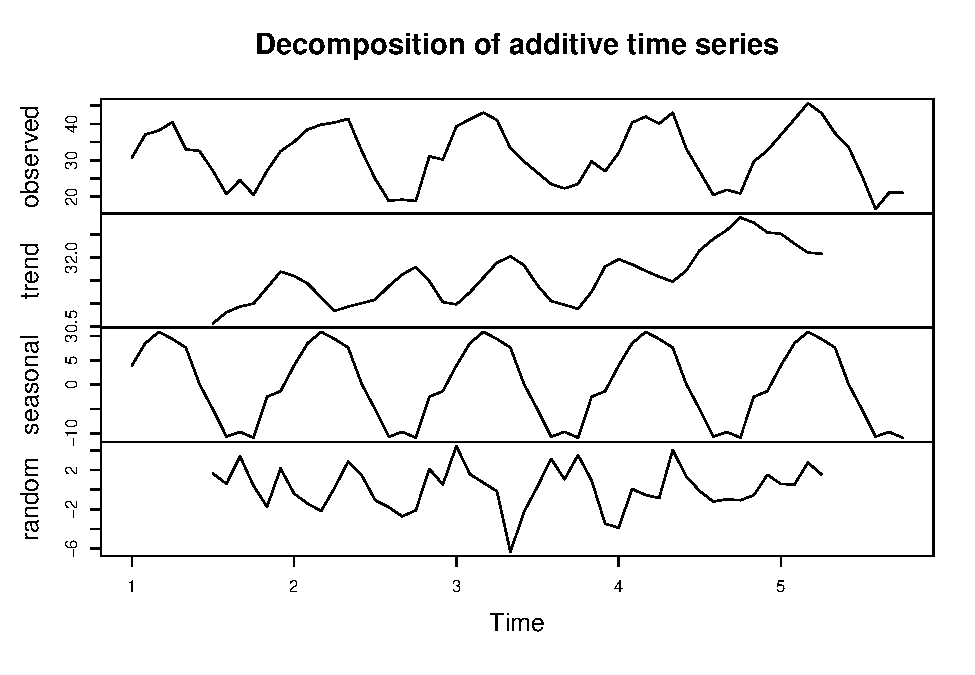
\includegraphics{timeSeries_files/figure-latex/unnamed-chunk-6-1.pdf}

Observamos en la gráfica:\\
-los valores de la serie\\
-la tendencia calculada mediante filtros\\
-la estacionalidad repetida cada 12 instantes de tiempo -lo que queda de
la serie al eliminar tendencia y estacionalidad

Como vemos, es posible que exista una alta varianza en los datos sin
estacionalidad y tendencia, por lo que probamos a aplicar una
transformación logarítmica para evitar problemas a la hora de tener en
cuenta la estacionariedad, ya que sabemos que una serie con
estacionariedad no varía ni en media ni en varianza.

\begin{Shaded}
\begin{Highlighting}[]
\NormalTok{serie.ts.log =}\StringTok{ }\KeywordTok{log}\NormalTok{(serie.ts)}
\NormalTok{serie.log =}\StringTok{ }\KeywordTok{log}\NormalTok{(serie)}
\KeywordTok{plot}\NormalTok{(}\KeywordTok{decompose}\NormalTok{(serie.ts.log))}
\end{Highlighting}
\end{Shaded}

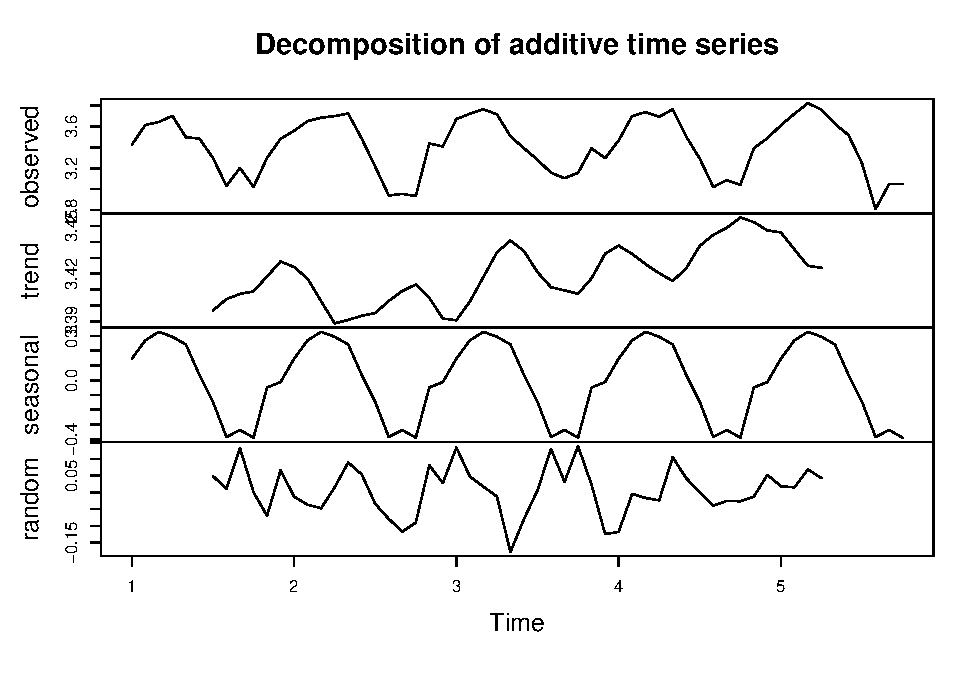
\includegraphics{timeSeries_files/figure-latex/unnamed-chunk-7-1.pdf}

De forma ligera, la varianza disminuye a lo largo del tiempo, lo que
producirá menores problemas a la hora de calcular la estacionariedad.
Por simplicidad usare la variable serie como serie.log (con la
transformación hecha)

\begin{Shaded}
\begin{Highlighting}[]
\NormalTok{serie =}\StringTok{ }\NormalTok{serie.log}
\end{Highlighting}
\end{Shaded}

Observamos como el atributo seasonal que nos da la función decompose
consta de los mismos valores para cada año de todos los meses, lo cual
nos dará la capacidad de calcular la estacionalidad para restársela a la
serie.

\begin{Shaded}
\begin{Highlighting}[]
\KeywordTok{decompose}\NormalTok{(serie.ts.log)}\OperatorTok{$}\NormalTok{seasonal}
\end{Highlighting}
\end{Shaded}

\begin{verbatim}
##           Jan         Feb         Mar         Apr         May         Jun
## 1  0.14624562  0.27038082  0.32826498  0.29462730  0.24274200  0.03660037
## 2  0.14624562  0.27038082  0.32826498  0.29462730  0.24274200  0.03660037
## 3  0.14624562  0.27038082  0.32826498  0.29462730  0.24274200  0.03660037
## 4  0.14624562  0.27038082  0.32826498  0.29462730  0.24274200  0.03660037
## 5  0.14624562  0.27038082  0.32826498  0.29462730  0.24274200  0.03660037
##           Jul         Aug         Sep         Oct         Nov         Dec
## 1 -0.14645133 -0.38469232 -0.33717450 -0.38909044 -0.04904490 -0.01240760
## 2 -0.14645133 -0.38469232 -0.33717450 -0.38909044 -0.04904490 -0.01240760
## 3 -0.14645133 -0.38469232 -0.33717450 -0.38909044 -0.04904490 -0.01240760
## 4 -0.14645133 -0.38469232 -0.33717450 -0.38909044 -0.04904490 -0.01240760
## 5 -0.14645133 -0.38469232 -0.33717450 -0.38909044
\end{verbatim}

Calculamos los instantes de tiempo de la serie para train y para test

\begin{Shaded}
\begin{Highlighting}[]
\CommentTok{# para train}
\NormalTok{tiempo =}\StringTok{ }\DecValTok{1}\OperatorTok{:}\KeywordTok{length}\NormalTok{(serie)}
\CommentTok{# para test}
\NormalTok{tiempoTs =}\StringTok{ }\NormalTok{(tiempo[}\KeywordTok{length}\NormalTok{(tiempo)]}\OperatorTok{+}\DecValTok{1}\NormalTok{)}\OperatorTok{:}\NormalTok{(tiempo[}\KeywordTok{length}\NormalTok{(tiempo)]}\OperatorTok{+}\NormalTok{Npred)}
\end{Highlighting}
\end{Shaded}

Representamos a continuación la serie que tenemos en este momento:

\begin{Shaded}
\begin{Highlighting}[]
\KeywordTok{plot.ts}\NormalTok{(serie,  }\DataTypeTok{xlim=}\KeywordTok{c}\NormalTok{(}\DecValTok{1}\NormalTok{, tiempoTs[}\KeywordTok{length}\NormalTok{(tiempoTs)]))}
\end{Highlighting}
\end{Shaded}

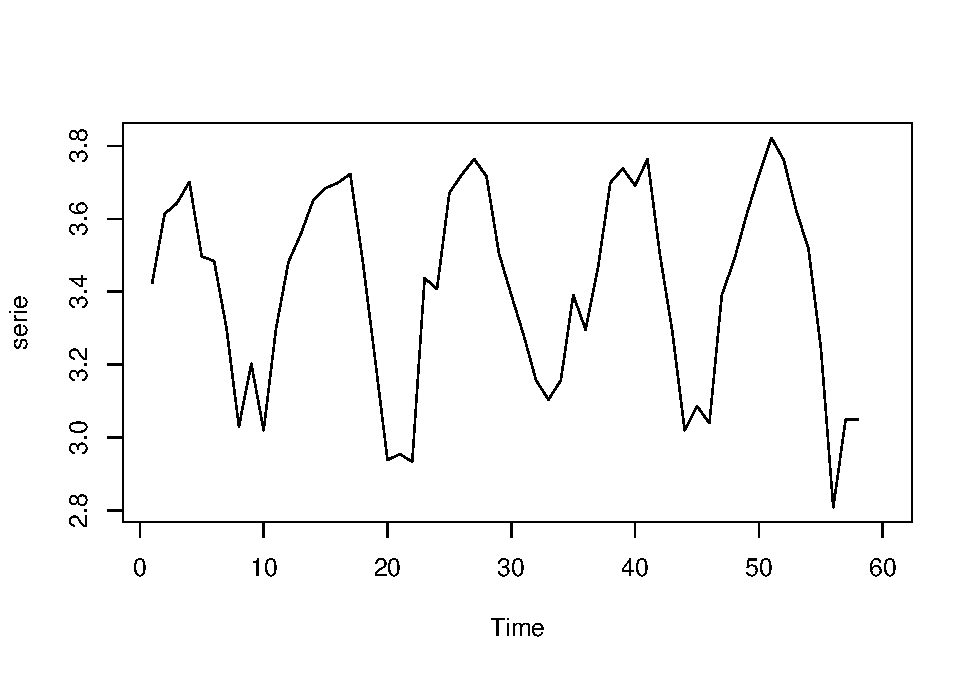
\includegraphics{timeSeries_files/figure-latex/unnamed-chunk-11-1.pdf}

Modelamos la tendencia, la cual podemos aparentemente ajustarla de forma
lineal, sabiendo que:\\
serie = parametroA * tiempo + parametroB\\
Con ayuda de la función lm calculamos dichos parámetros:

\begin{Shaded}
\begin{Highlighting}[]
\NormalTok{parametros.H1 =}\StringTok{ }\KeywordTok{lm}\NormalTok{(serie }\OperatorTok{~}\NormalTok{tiempo)}
\NormalTok{parametros.H1}
\end{Highlighting}
\end{Shaded}

\begin{verbatim}
## 
## Call:
## lm(formula = serie ~ tiempo)
## 
## Coefficients:
## (Intercept)       tiempo  
##    3.451367    -0.001317
\end{verbatim}

Tomamos Intercept como termino independiente (parametroB) y el otro como
el que multiplica al tiempo para poder calcular la serie (parametroA).
Para modelar la tendencia usamos la fórmula descrita antes:

\begin{Shaded}
\begin{Highlighting}[]
\CommentTok{# tendencia estimada para los datos de train}
\NormalTok{tendEstimadaTr =}\StringTok{  }\NormalTok{parametros.H1}\OperatorTok{$}\NormalTok{coefficients[}\DecValTok{1}\NormalTok{] }\OperatorTok{+}\StringTok{ }\NormalTok{tiempo}\OperatorTok{*}\NormalTok{parametros.H1}\OperatorTok{$}\NormalTok{coefficients[}\DecValTok{2}\NormalTok{] }
\CommentTok{# tendencia estimada para las predicciones de test}
\NormalTok{tendEstimadaTs =}\StringTok{  }\NormalTok{parametros.H1}\OperatorTok{$}\NormalTok{coefficients[}\DecValTok{1}\NormalTok{] }\OperatorTok{+}\StringTok{ }\NormalTok{tiempoTs}\OperatorTok{*}\NormalTok{parametros.H1}\OperatorTok{$}\NormalTok{coefficients[}\DecValTok{2}\NormalTok{] }
\end{Highlighting}
\end{Shaded}

Comprobamos visualmente si la tendencia se ajusta al modelo que tenemos
de la serie temporal:

\begin{Shaded}
\begin{Highlighting}[]
\KeywordTok{plot.ts}\NormalTok{(serie, }\DataTypeTok{xlim=}\KeywordTok{c}\NormalTok{(}\DecValTok{1}\NormalTok{, tiempoTs[}\KeywordTok{length}\NormalTok{(tiempoTs)])) }
\KeywordTok{lines}\NormalTok{(tiempo, tendEstimadaTr, }\DataTypeTok{col =} \StringTok{"blue"}\NormalTok{) }
\KeywordTok{lines}\NormalTok{(tiempoTs, tendEstimadaTs, }\DataTypeTok{col =} \StringTok{"green"}\NormalTok{)}
\end{Highlighting}
\end{Shaded}

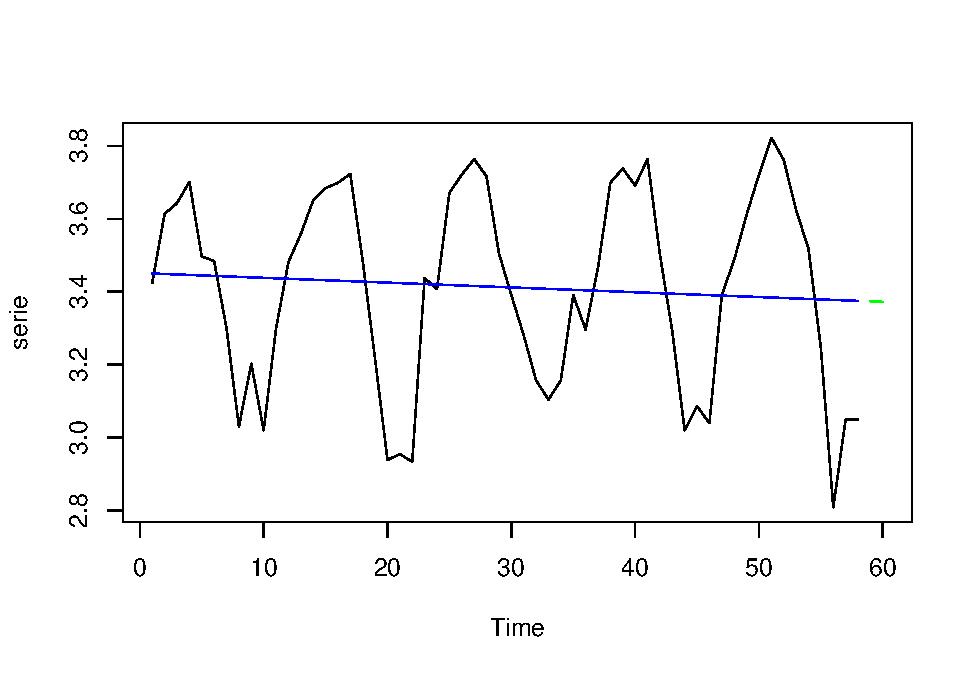
\includegraphics{timeSeries_files/figure-latex/unnamed-chunk-14-1.pdf}

Validamos de forma estadística que el modelo lineal sea correcto,
comprobando que los errores a lo largo de la serie se distribuyen
mediante una distribución normal. Para ello aplicamos el test de
Jarque-Bera:

\begin{Shaded}
\begin{Highlighting}[]
\NormalTok{JB =}\StringTok{ }\KeywordTok{jarque.bera.test}\NormalTok{(parametros.H1}\OperatorTok{$}\NormalTok{residuals)}
\NormalTok{JB}
\end{Highlighting}
\end{Shaded}

\begin{verbatim}
## 
##  Jarque Bera Test
## 
## data:  parametros.H1$residuals
## X-squared = 3.6086, df = 2, p-value = 0.1646
\end{verbatim}

Podemos asumir, con una confianza del 95\%, que no hay diferencia
significativa de los datos de error con respecto a los de una
distribución normal, debido a que el p-value es mayor que 0.05.

Procedemos por tanto a eliminar la tendencia de la serie actual:

\begin{Shaded}
\begin{Highlighting}[]
\NormalTok{serie.sinTend =}\StringTok{ }\NormalTok{serie }\OperatorTok{-}\StringTok{ }\NormalTok{tendEstimadaTr}
\end{Highlighting}
\end{Shaded}

Comprobamos como queda la serie sin tendencia:

\begin{Shaded}
\begin{Highlighting}[]
\KeywordTok{plot.ts}\NormalTok{(serie.sinTend, }\DataTypeTok{xlim=}\KeywordTok{c}\NormalTok{(}\DecValTok{1}\NormalTok{, tiempoTs[}\KeywordTok{length}\NormalTok{(tiempoTs)])) }
\end{Highlighting}
\end{Shaded}

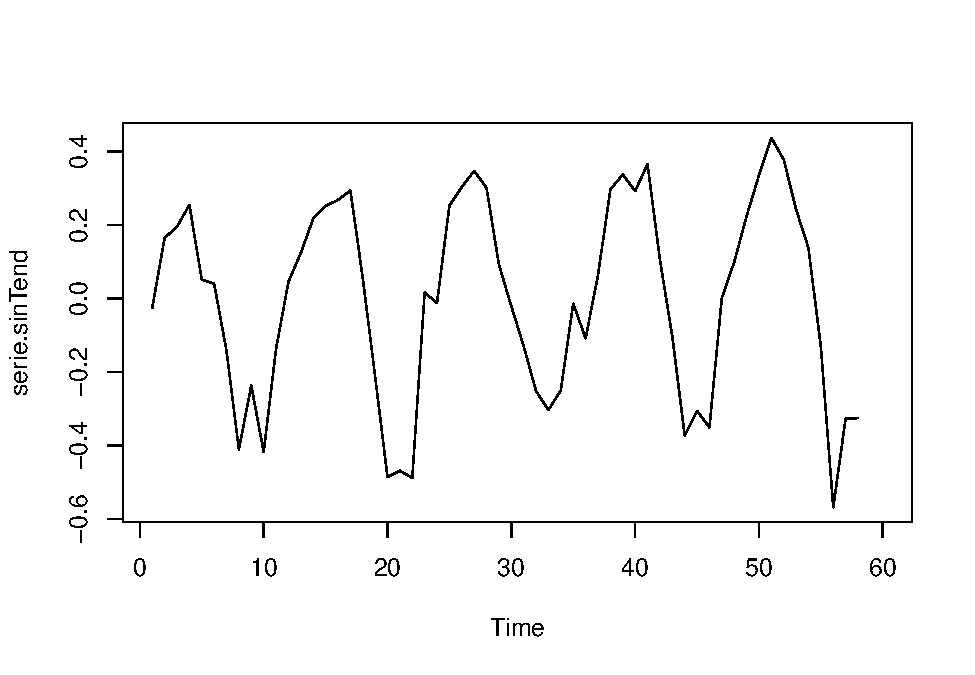
\includegraphics{timeSeries_files/figure-latex/unnamed-chunk-17-1.pdf}

Como vemos, la serie sin tendencia prácticamente es la misma que con
ella, ya que la pendiente del modelo lineal creado para el cálculo de
ésta era ínfima.

Procedemos, una vez eliminada la tendencia, a deshacernos de la
estacionalidad con ayuda de la función decompose.

\begin{Shaded}
\begin{Highlighting}[]
\NormalTok{k =}\StringTok{ }\DecValTok{12} \CommentTok{# aquí guardamos los datos estacionales}
\NormalTok{estacionalidad =}\StringTok{ }\KeywordTok{decompose}\NormalTok{(serie.ts.log)}\OperatorTok{$}\NormalTok{seasonal[}\DecValTok{1}\OperatorTok{:}\NormalTok{k]}
\end{Highlighting}
\end{Shaded}

Eliminamos dicha estacionalidad a la serie.

\begin{Shaded}
\begin{Highlighting}[]
\NormalTok{serie.sinTend.sinEst =}\StringTok{ }\NormalTok{serie.sinTend }\OperatorTok{-}\StringTok{ }\NormalTok{estacionalidad}
\end{Highlighting}
\end{Shaded}

\begin{verbatim}
## Warning in serie.sinTend - estacionalidad: longitud de objeto mayor no es
## múltiplo de la longitud de uno menor
\end{verbatim}

Comprobamos como se queda la serie sin dicha estacionalidad

\begin{Shaded}
\begin{Highlighting}[]
\KeywordTok{plot.ts}\NormalTok{(serie.sinTend.sinEst, }\DataTypeTok{xlim=}\KeywordTok{c}\NormalTok{(}\DecValTok{1}\NormalTok{, tiempoTs[}\KeywordTok{length}\NormalTok{(tiempoTs)])) }
\end{Highlighting}
\end{Shaded}

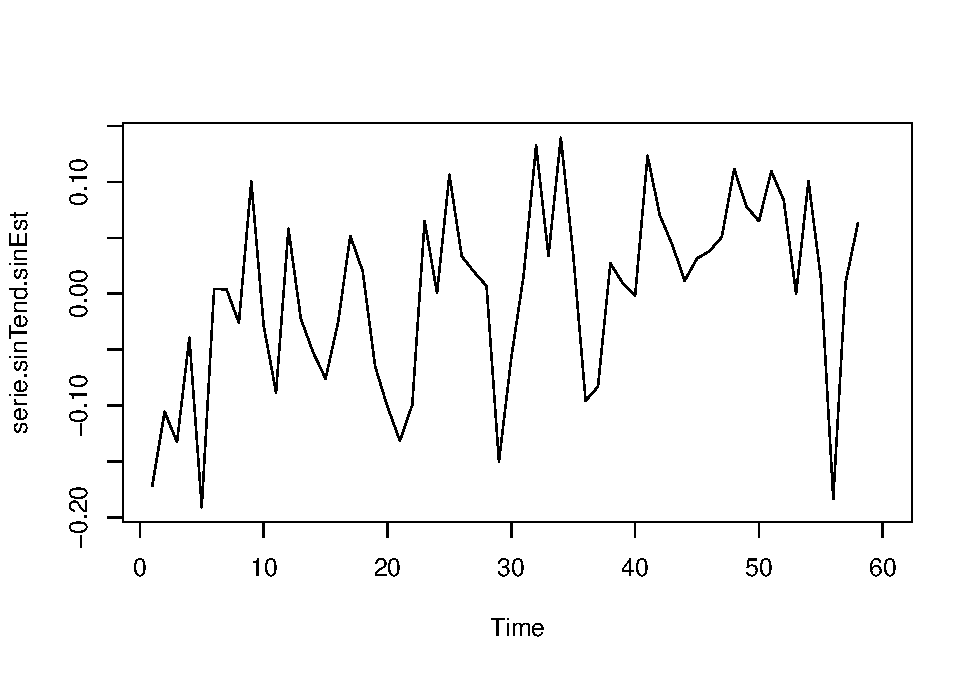
\includegraphics{timeSeries_files/figure-latex/unnamed-chunk-20-1.pdf}

Ahora que tan solo nos queda la componente irregular tras haber
eliminado las componentes de tendencia y estacionalidad, procedemos a
comprobar si la serie es estacionaria o no mediante el test ACF.

\begin{Shaded}
\begin{Highlighting}[]
\KeywordTok{acf}\NormalTok{(serie.sinTend.sinEst)}
\end{Highlighting}
\end{Shaded}

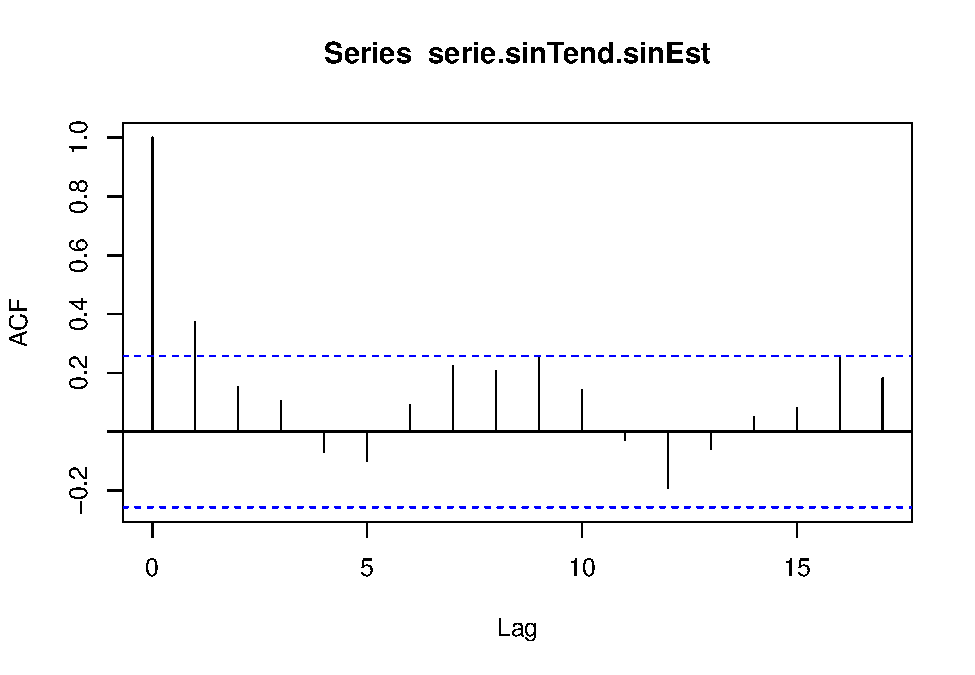
\includegraphics{timeSeries_files/figure-latex/unnamed-chunk-21-1.pdf}

A priori parece ser, debido a la rapidez de bajada entre instantes de
tiempo y a la estabilización en forma de `'olas'', que existe una clara
estacionariedad. Aun así, probaré aplicar el test de Dickey-Fuller
aumentado para asegurarnos de ello.

\begin{Shaded}
\begin{Highlighting}[]
\KeywordTok{adf.test}\NormalTok{(serie.sinTend.sinEst)}
\end{Highlighting}
\end{Shaded}

\begin{verbatim}
## Warning in adf.test(serie.sinTend.sinEst): p-value smaller than printed p-
## value
\end{verbatim}

\begin{verbatim}
## 
##  Augmented Dickey-Fuller Test
## 
## data:  serie.sinTend.sinEst
## Dickey-Fuller = -4.9184, Lag order = 3, p-value = 0.01
## alternative hypothesis: stationary
\end{verbatim}

Al tomar como hipótesis nula que la serie es estacionaria y al ser el
p-value inferior a 0.05, podemos asegurar con un 95\% de probabilidad
que la serie es estacionaria, por tanto la tomamos así. Debido a esto no
será necesario realizar diferenciación para convertir la serie en
estacionaria.

Observamos el acf parcial para ver como influyen de forma individual
cada uno de los instantes de tiempo sobre el instante actual.

\begin{Shaded}
\begin{Highlighting}[]
\KeywordTok{pacf}\NormalTok{(serie.sinTend.sinEst)}
\end{Highlighting}
\end{Shaded}

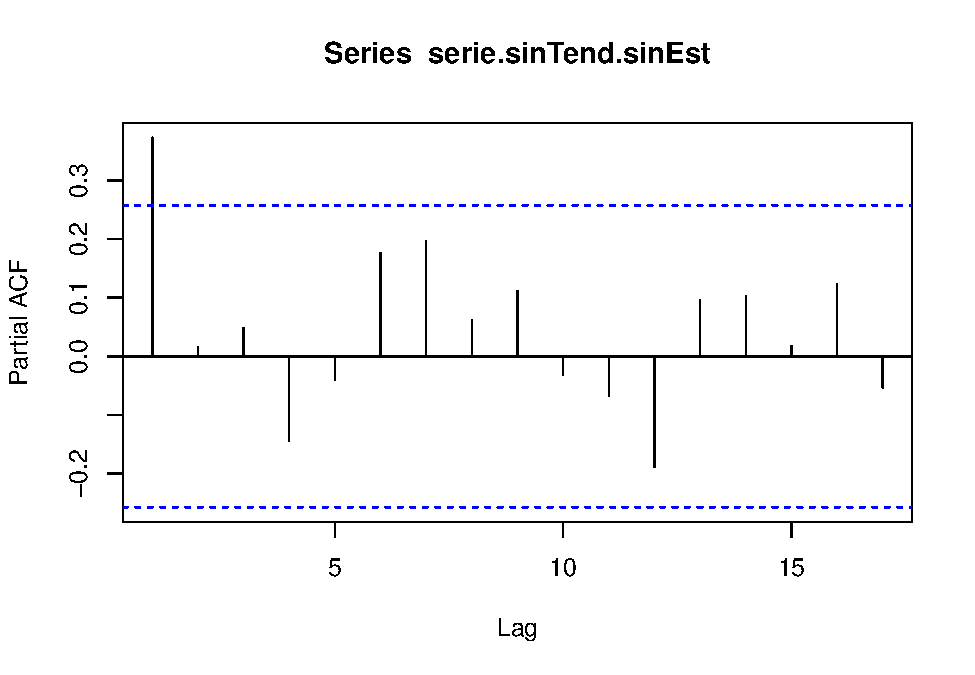
\includegraphics{timeSeries_files/figure-latex/unnamed-chunk-23-1.pdf}

A la vista de las gráficas ofrecidas por ACF y PACF, me resulta de mayor
claridad decidirme por un modelo autoregresivo en lugar de uno de medias
móviles debido a que en ACF los valores de cada instante son más altos y
sobrepasan los límites más que los de PACF, además de que se ve de forma
mucho más clara esa estabilización en forma de `'olas'' que he dicho
anteriormente en la gráfica del ACF. Por ello mismo, deberíamos poder
modelar la componente irregular de la serie con un modelo autoregresivo
de orden 0 (fijándonos en la gráfica PACF), utilizando un modelo ARIMA
con cero diferenciaciones. Entrenamos dicho modelo a continuación:

\begin{Shaded}
\begin{Highlighting}[]
\CommentTok{# coeficiente de autoregresión = 0, diferenciaciones = 0, coeficiente de medias moviles = 0}
\NormalTok{modelo =}\StringTok{ }\KeywordTok{arima}\NormalTok{(serie.sinTend.sinEst, }\DataTypeTok{order =} \KeywordTok{c}\NormalTok{(}\DecValTok{0}\NormalTok{,}\DecValTok{0}\NormalTok{,}\DecValTok{0}\NormalTok{))}

\CommentTok{# calculamos las predicciones}
\NormalTok{predicciones =}\StringTok{ }\KeywordTok{predict}\NormalTok{(modelo, }\DataTypeTok{n.ahead =}\NormalTok{ Npred)}
\NormalTok{valoresPredichos =}\StringTok{ }\NormalTok{predicciones}\OperatorTok{$}\NormalTok{pred}
\NormalTok{valoresPredichos}
\end{Highlighting}
\end{Shaded}

\begin{verbatim}
## Time Series:
## Start = 59 
## End = 60 
## Frequency = 1 
## [1] -0.001059526 -0.001059526
\end{verbatim}

Observamos ahora de forma visual el modelo incluyendo la serie sin
tendencia ni estacionalidad

\begin{Shaded}
\begin{Highlighting}[]
\KeywordTok{plot.ts}\NormalTok{(serie.sinTend.sinEst, }\DataTypeTok{xlim=}\KeywordTok{c}\NormalTok{(}\DecValTok{1}\NormalTok{, tiempoTs[}\KeywordTok{length}\NormalTok{(tiempoTs)])) }
\KeywordTok{lines}\NormalTok{(tiempoTs,valoresPredichos, }\DataTypeTok{col=}\StringTok{"green"}\NormalTok{)}
\end{Highlighting}
\end{Shaded}

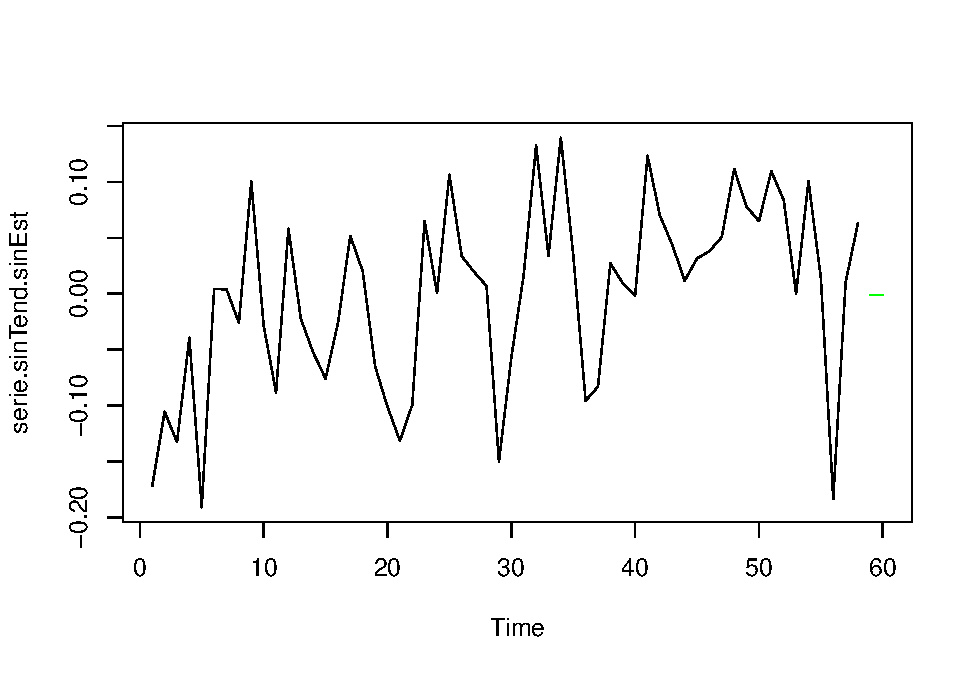
\includegraphics{timeSeries_files/figure-latex/unnamed-chunk-25-1.pdf}

Parece ser que los resultados obtenidos no son buenamente fieles a lo
esperado, quizás debido a la cercanía de los valores en los sucesivos
instantes de tiempo en las gráficas ACF y PACF. Visto lo visto, puede
decirse que nuestra serie es prácticamente ruido blanco debido a los
resultados obtenidos como predicciones.\\
Finalmente probamos la validez de nuestro modelo (sus errores) mediante
tests estadísticos. Aplicamos varios:

Test de Box-Pierce: comprobamos que los residuos que nos quedan son
aleatorios:

\begin{Shaded}
\begin{Highlighting}[]
\KeywordTok{Box.test}\NormalTok{(modelo}\OperatorTok{$}\NormalTok{residuals)}
\end{Highlighting}
\end{Shaded}

\begin{verbatim}
## 
##  Box-Pierce test
## 
## data:  modelo$residuals
## X-squared = 8.0586, df = 1, p-value = 0.004529
\end{verbatim}

Tras este test comprobamos que los errores obtenidos no son de forma
aleatoria, por lo que el modelo arima creado no es correcto. Debido a
esto, probaré el ajuste de un modelo de medias móviles de grado 1 (el
grado determinado por la gráfica ACF) para comprobar su validez:

\begin{Shaded}
\begin{Highlighting}[]
\CommentTok{# coeficiente de autoregresión = 0, diferenciaciones = 0, coeficiente de medias moviles = 1}
\NormalTok{modelo =}\StringTok{ }\KeywordTok{arima}\NormalTok{(serie.sinTend.sinEst, }\DataTypeTok{order =} \KeywordTok{c}\NormalTok{(}\DecValTok{0}\NormalTok{,}\DecValTok{0}\NormalTok{,}\DecValTok{1}\NormalTok{))}

\CommentTok{# calculamos las predicciones}
\NormalTok{predicciones =}\StringTok{ }\KeywordTok{predict}\NormalTok{(modelo, }\DataTypeTok{n.ahead =}\NormalTok{ Npred)}
\NormalTok{valoresPredichos =}\StringTok{ }\NormalTok{predicciones}\OperatorTok{$}\NormalTok{pred}
\NormalTok{valoresPredichos}
\end{Highlighting}
\end{Shaded}

\begin{verbatim}
## Time Series:
## Start = 59 
## End = 60 
## Frequency = 1 
## [1]  0.011869071 -0.001802729
\end{verbatim}

Observamos los valores predichos con el modelo de medias móviles con la
serie sin tendencia ni estacionalidad:

\begin{Shaded}
\begin{Highlighting}[]
\KeywordTok{plot.ts}\NormalTok{(serie.sinTend.sinEst, }\DataTypeTok{xlim=}\KeywordTok{c}\NormalTok{(}\DecValTok{1}\NormalTok{, tiempoTs[}\KeywordTok{length}\NormalTok{(tiempoTs)])) }
\KeywordTok{lines}\NormalTok{(tiempoTs,valoresPredichos, }\DataTypeTok{col=}\StringTok{"green"}\NormalTok{)}
\end{Highlighting}
\end{Shaded}

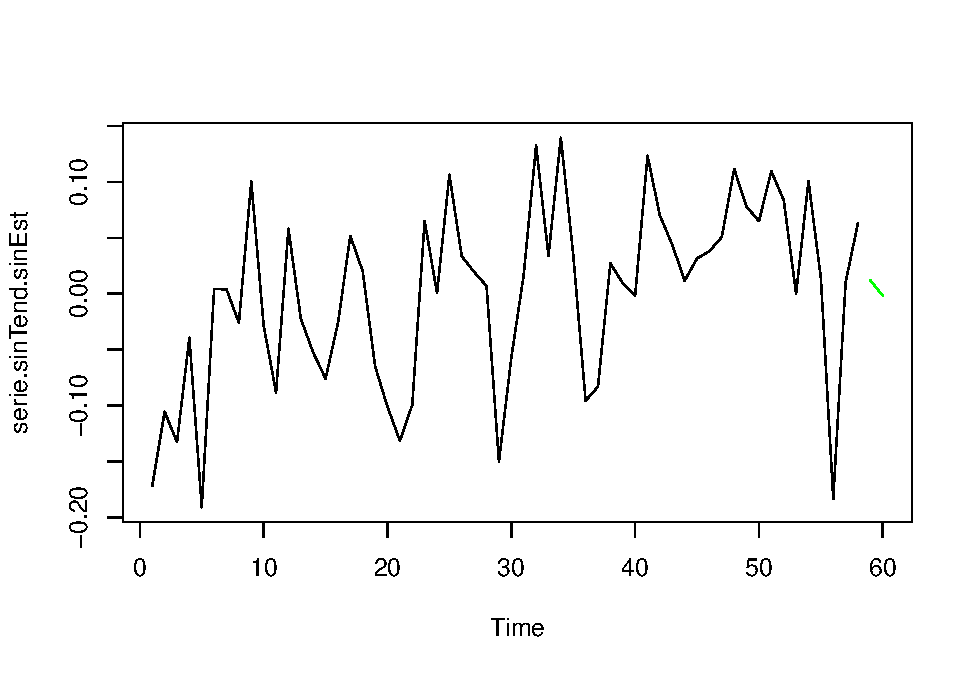
\includegraphics{timeSeries_files/figure-latex/unnamed-chunk-28-1.pdf}
Aplicamos de nuevo el test de Box-Pierce para la comprobación de la
aleatoriedad de los errores:

\begin{Shaded}
\begin{Highlighting}[]
\KeywordTok{Box.test}\NormalTok{(modelo}\OperatorTok{$}\NormalTok{residuals)}
\end{Highlighting}
\end{Shaded}

\begin{verbatim}
## 
##  Box-Pierce test
## 
## data:  modelo$residuals
## X-squared = 0.0086579, df = 1, p-value = 0.9259
\end{verbatim}

Este valor de p-value nos dice con un 95\% de confianza que los errores
obtenidos por el modelo creado son aleatorios, por lo que el modelo
queda validado por este test.

Continuamos con los tests de normalidad.

Jarque Bera: vemos si los residuos, aunque aleatorios, son normales
(media cero y desviación típica la que sea).

\begin{Shaded}
\begin{Highlighting}[]
\KeywordTok{jarque.bera.test}\NormalTok{(modelo}\OperatorTok{$}\NormalTok{residuals) }
\end{Highlighting}
\end{Shaded}

\begin{verbatim}
## 
##  Jarque Bera Test
## 
## data:  modelo$residuals
## X-squared = 1.3191, df = 2, p-value = 0.5171
\end{verbatim}

Saphiro-Wilk: mismo cometido que Jarque Bera

\begin{Shaded}
\begin{Highlighting}[]
 \KeywordTok{shapiro.test}\NormalTok{(modelo}\OperatorTok{$}\NormalTok{residuals) }
\end{Highlighting}
\end{Shaded}

\begin{verbatim}
## 
##  Shapiro-Wilk normality test
## 
## data:  modelo$residuals
## W = 0.9788, p-value = 0.4025
\end{verbatim}

Asumimos tras la ejecución de ambos tests que los residuos siguen una
distribuición normal debido a los p-values obtenidos, ya que la
hipótesis nula propone que los datos no siguen una distribución normal.

A continuación obtenemos un histograma y función de densidad para
obtener resultados gráficos de confirmación.

\begin{Shaded}
\begin{Highlighting}[]
\KeywordTok{hist}\NormalTok{(modelo}\OperatorTok{$}\NormalTok{residuals, }\DataTypeTok{col=}\StringTok{"blue"}\NormalTok{, }\DataTypeTok{prob=}\NormalTok{T,}\DataTypeTok{ylim=}\KeywordTok{c}\NormalTok{(}\DecValTok{0}\NormalTok{,}\DecValTok{20}\NormalTok{), }\DataTypeTok{xlim=}\KeywordTok{c}\NormalTok{(}\OperatorTok{-}\FloatTok{0.2}\NormalTok{,}\FloatTok{0.2}\NormalTok{))}
\KeywordTok{lines}\NormalTok{(}\KeywordTok{density}\NormalTok{(modelo}\OperatorTok{$}\NormalTok{residuals))}
\end{Highlighting}
\end{Shaded}

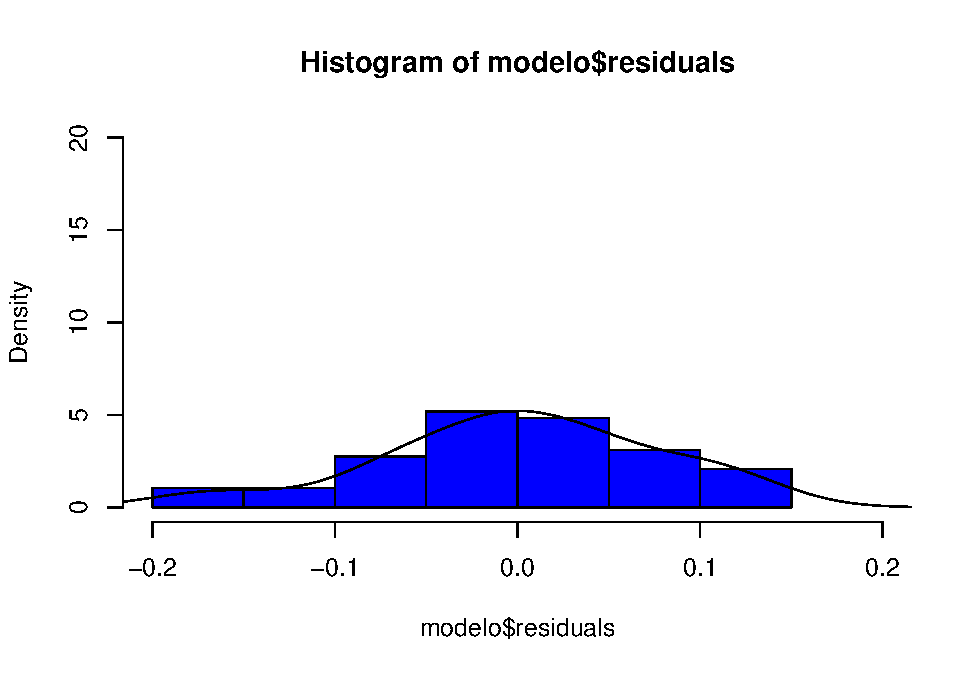
\includegraphics{timeSeries_files/figure-latex/unnamed-chunk-32-1.pdf}

Con estas comprobaciones el modelo queda validado, ya que los errores
que nos dan son aleatorios que provienen de una distribución normal. A
continuación hemos de deshacer los cambios para obtener los predicciones
reales:

\begin{Shaded}
\begin{Highlighting}[]
\NormalTok{estacionalidades =}\StringTok{ }\KeywordTok{c}\NormalTok{(estacionalidad[}\DecValTok{11}\NormalTok{], estacionalidad[}\DecValTok{12}\NormalTok{])}

\CommentTok{# Incluimos la estacionalidad }
\NormalTok{valoresPredichos.Est =}\StringTok{ }\NormalTok{valoresPredichos }\OperatorTok{+}\StringTok{ }\NormalTok{estacionalidades}

\CommentTok{# Incluimos la tendencia }
\NormalTok{valoresPredichos.Est.Tend =}\StringTok{ }\NormalTok{valoresPredichos.Est }\OperatorTok{+}\StringTok{ }\NormalTok{tendEstimadaTs}

\CommentTok{# Transformación de los logaritmos }
\NormalTok{valoresPredichos.Est.Tend.exp =}\StringTok{ }\KeywordTok{exp}\NormalTok{(valoresPredichos.Est.Tend)}

\CommentTok{# usamos exp(serie) por haber hecho al principio serie = log(serie)}
\KeywordTok{plot.ts}\NormalTok{(}\KeywordTok{exp}\NormalTok{(serie),}\DataTypeTok{xlim=}\KeywordTok{c}\NormalTok{(}\DecValTok{1}\NormalTok{, tiempoTs[}\KeywordTok{length}\NormalTok{(tiempoTs)])) }
\KeywordTok{lines}\NormalTok{(tiempoTs, valoresPredichos.Est.Tend.exp, }\DataTypeTok{col =} \StringTok{"green"}\NormalTok{)}
\end{Highlighting}
\end{Shaded}

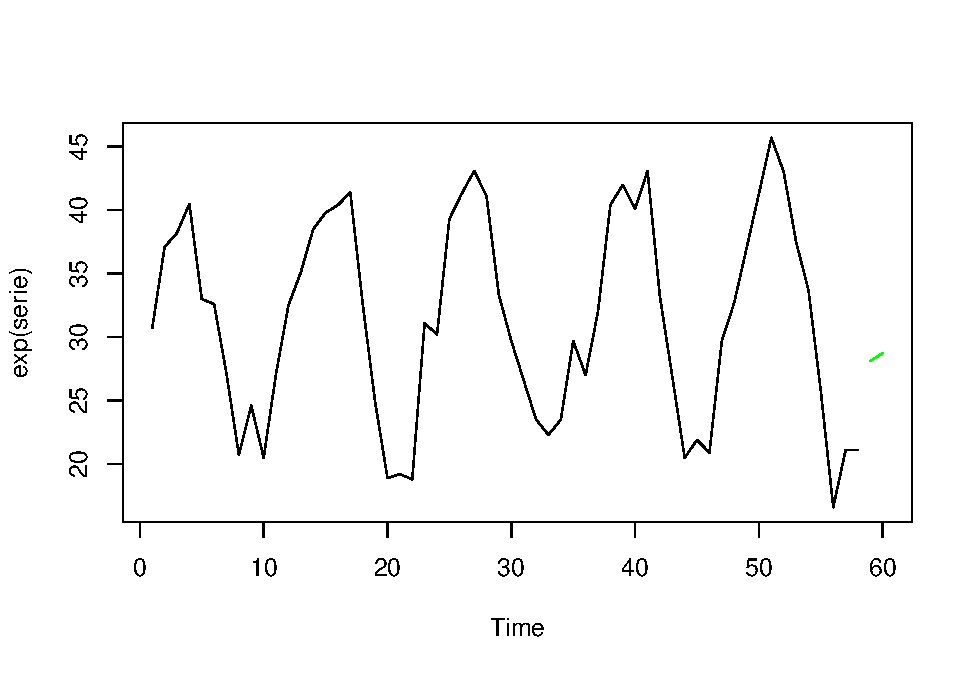
\includegraphics{timeSeries_files/figure-latex/unnamed-chunk-33-1.pdf}

Finalmente podemos observar en la gráfica los valores de temperatura
máxima obtenidos para los meses de Marzo y Abril de 2018, los cuales se
corresponden respectivamente con los valores:

\begin{Shaded}
\begin{Highlighting}[]
\NormalTok{valoresPredichos.Est.Tend.exp}
\end{Highlighting}
\end{Shaded}

\begin{verbatim}
## Time Series:
## Start = 59 
## End = 60 
## Frequency = 1 
## [1] 28.12089 28.73632
\end{verbatim}

\section{Problema 2.  ¿Qué valores de temperatura máxima, a escala diaria, se espera para la primera semana de Marzo de 2018?}

Primeramente leemos el conjunto de datos que contiene los siguientes
atributos:\\
- Columna 1 : Identificador Estación\\
- Columna 2 : Fecha\\
- Columna 3 : Temperatura Máxima (ºC)\\
- Columna 4 : Hora Temperatura Máxima\\
- Columna 5 : Temperatura mínima (ºC)\\
- Columna 6 : Hora Temperatura mínima\\
- Columna 7 : Temperatura Media (ºC)\\
- Columna 8 : Racha máxima de viento (Km/h)\\
- Columna 9 : Hora de Racha Máxima\\
- Columna 10 : Velocidad media de Viento (Km/h)\\
- Columna 11 : Hora de Velocidad Máxima de viento\\
- Columna 12 : Precipitacion Total diaria (mm)\\
- Columna 13 : Precipitacion de 0 a 6 horas (mm)\\
- Columna 14 : Precipitacion de 6 a 12 horas (mm)\\
- Columna 15 : Precipitacion de 12 a 18 horas (mm)\\
- Columna 16 : Precipitacion de 18 a 24 horas (mm)

Librerías\ldots{}

\begin{Shaded}
\begin{Highlighting}[]
\KeywordTok{library}\NormalTok{(tseries)}
\KeywordTok{library}\NormalTok{(dplyr)}
\KeywordTok{library}\NormalTok{(lubridate)}
\KeywordTok{library}\NormalTok{(imputeTS)}
\end{Highlighting}
\end{Shaded}

\begin{verbatim}
## 
## Attaching package: 'imputeTS'
\end{verbatim}

\begin{verbatim}
## The following object is masked from 'package:tseries':
## 
##     na.remove
\end{verbatim}

Leemos el dataset y, como solo nos interesa la fecha y la temperatura
máxima nos quedamos con tan solo esos datos.

\begin{Shaded}
\begin{Highlighting}[]
\NormalTok{datos =}\StringTok{ }\KeywordTok{read.csv}\NormalTok{(}\StringTok{"5530E.csv"}\NormalTok{, }\DataTypeTok{header =} \OtherTok{TRUE}\NormalTok{, }\DataTypeTok{sep=}\StringTok{";"}\NormalTok{)}
\NormalTok{datos =}\StringTok{ }\NormalTok{datos[,}\KeywordTok{c}\NormalTok{(}\StringTok{"Fecha"}\NormalTok{,}\StringTok{"Tmax"}\NormalTok{)]}
\NormalTok{datos}\OperatorTok{$}\NormalTok{Fecha =}\StringTok{ }\KeywordTok{as.Date}\NormalTok{(datos}\OperatorTok{$}\NormalTok{Fecha)}
\end{Highlighting}
\end{Shaded}

Veamos los valores NA\ldots{}

\begin{Shaded}
\begin{Highlighting}[]
\KeywordTok{apply}\NormalTok{(datos, }\DecValTok{2}\NormalTok{, }\ControlFlowTok{function}\NormalTok{(atributo)\{}\KeywordTok{sum}\NormalTok{(}\KeywordTok{is.na}\NormalTok{(atributo))\})}
\end{Highlighting}
\end{Shaded}

\begin{verbatim}
## Fecha  Tmax 
##     0   124
\end{verbatim}

Imputamos valores mediante interpolación en las temperaturas máximas
donde existan valores perdidos con el fin de no tergiversar los datos
eliminando días del año.

\begin{Shaded}
\begin{Highlighting}[]
\NormalTok{datos}\OperatorTok{$}\NormalTok{Tmax =}\StringTok{ }\KeywordTok{na.interpolation}\NormalTok{(datos}\OperatorTok{$}\NormalTok{Tmax)}
\end{Highlighting}
\end{Shaded}

Obtenemos ahora la cantidad de datos a predecir y la serie temporal en
sí

\begin{Shaded}
\begin{Highlighting}[]
\NormalTok{Npred =}\StringTok{ }\DecValTok{7} \CommentTok{# cantidad de datos a predecir (temperaturas máximas de marzo y abril)}
\NormalTok{serie =}\StringTok{ }\NormalTok{datos}\OperatorTok{$}\NormalTok{Tmax}
\NormalTok{serie.ts =}\StringTok{ }\KeywordTok{ts}\NormalTok{(serie, }\DataTypeTok{frequency =} \DecValTok{365}\NormalTok{) }\CommentTok{# frequency set to 12 to set stationality each 12 months}
\KeywordTok{plot}\NormalTok{(}\KeywordTok{decompose}\NormalTok{(serie.ts))}
\end{Highlighting}
\end{Shaded}

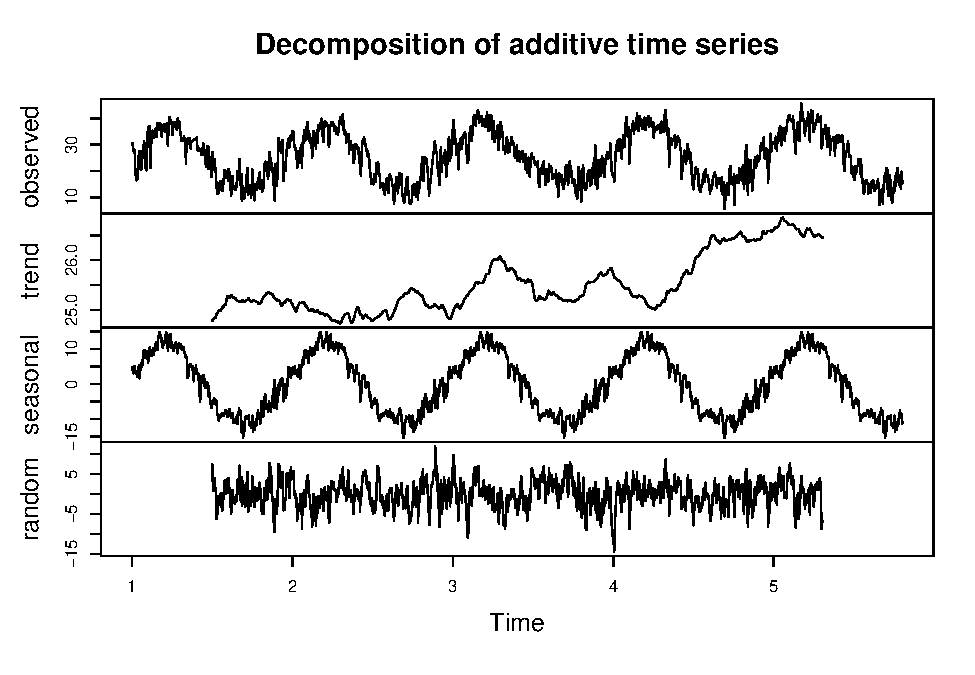
\includegraphics{timeSeries_files/figure-latex/unnamed-chunk-39-1.pdf}

Observamos en la gráfica:\\
-los valores de la serie\\
-la tendencia calculada mediante filtros\\
-la estacionalidad repetida cada 12 instantes de tiempo -lo que queda de
la serie al eliminar tendencia y estacionalidad

Probamos, como hemos hecho en experimentos anteriores, a realizar una
transformación logarítmica de la serie para reducir la varianza y así
evitar problemas con el cálculo de la estacionariedad:

\begin{Shaded}
\begin{Highlighting}[]
\NormalTok{serie.ts.log =}\StringTok{ }\KeywordTok{log}\NormalTok{(serie.ts) }
\NormalTok{serie.log =}\StringTok{ }\KeywordTok{log}\NormalTok{(serie) }
\KeywordTok{plot}\NormalTok{(}\KeywordTok{decompose}\NormalTok{(serie.ts.log))}
\end{Highlighting}
\end{Shaded}

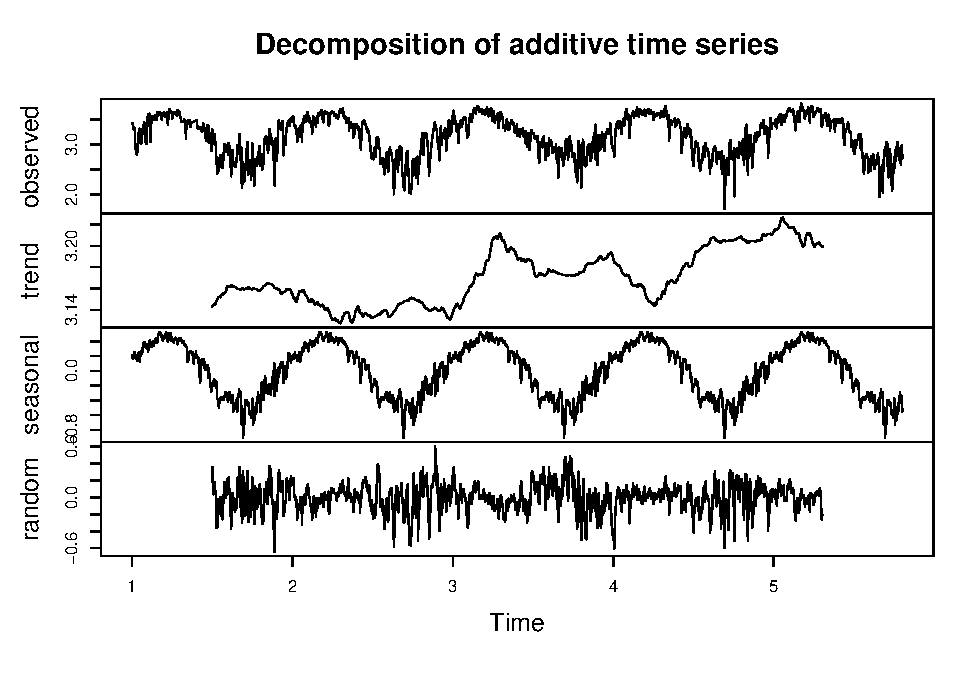
\includegraphics{timeSeries_files/figure-latex/unnamed-chunk-40-1.pdf}

El cambio es relativamente muy pequeño, es posible que tenga mucho que
ver la gran cantidad de datos, siendo difícil distinguir la variación
entre la gráfica anterior y esta. Aún así, por precaución, tomaremos
esta serie por válida.

Observamos los datos de estacionalidad que nos servirán en el futuro
para eliminársela a la serie temporal.

\begin{Shaded}
\begin{Highlighting}[]
\KeywordTok{head}\NormalTok{(}\KeywordTok{decompose}\NormalTok{(serie.ts.log)}\OperatorTok{$}\NormalTok{seasonal)}
\end{Highlighting}
\end{Shaded}

\begin{verbatim}
## Time Series:
## Start = c(1, 1) 
## End = c(1, 6) 
## Frequency = 365 
## [1] 0.1797105 0.2053683 0.1774451 0.1648794 0.1722653 0.2133311
\end{verbatim}

Por simplicidad en el uso de la nomenclatura utilizare la variable serie
en lugar de serie.log

\begin{Shaded}
\begin{Highlighting}[]
\NormalTok{serie =}\StringTok{ }\NormalTok{serie.log}
\end{Highlighting}
\end{Shaded}

Calculamos los instantes de tiempo de la serie

\begin{Shaded}
\begin{Highlighting}[]
\CommentTok{# para train}
\NormalTok{tiempo =}\StringTok{ }\DecValTok{1}\OperatorTok{:}\KeywordTok{length}\NormalTok{(serie.ts.log)}
\CommentTok{# para test}
\NormalTok{tiempoTs =}\StringTok{ }\NormalTok{(tiempo[}\KeywordTok{length}\NormalTok{(tiempo)]}\OperatorTok{+}\DecValTok{1}\NormalTok{)}\OperatorTok{:}\NormalTok{(tiempo[}\KeywordTok{length}\NormalTok{(tiempo)]}\OperatorTok{+}\NormalTok{Npred)}
\end{Highlighting}
\end{Shaded}

Representamos la serie

\begin{Shaded}
\begin{Highlighting}[]
\KeywordTok{plot.ts}\NormalTok{(serie, }\DataTypeTok{xlim=}\KeywordTok{c}\NormalTok{(}\DecValTok{1}\NormalTok{, tiempoTs[}\KeywordTok{length}\NormalTok{(tiempoTs)]))}
\end{Highlighting}
\end{Shaded}

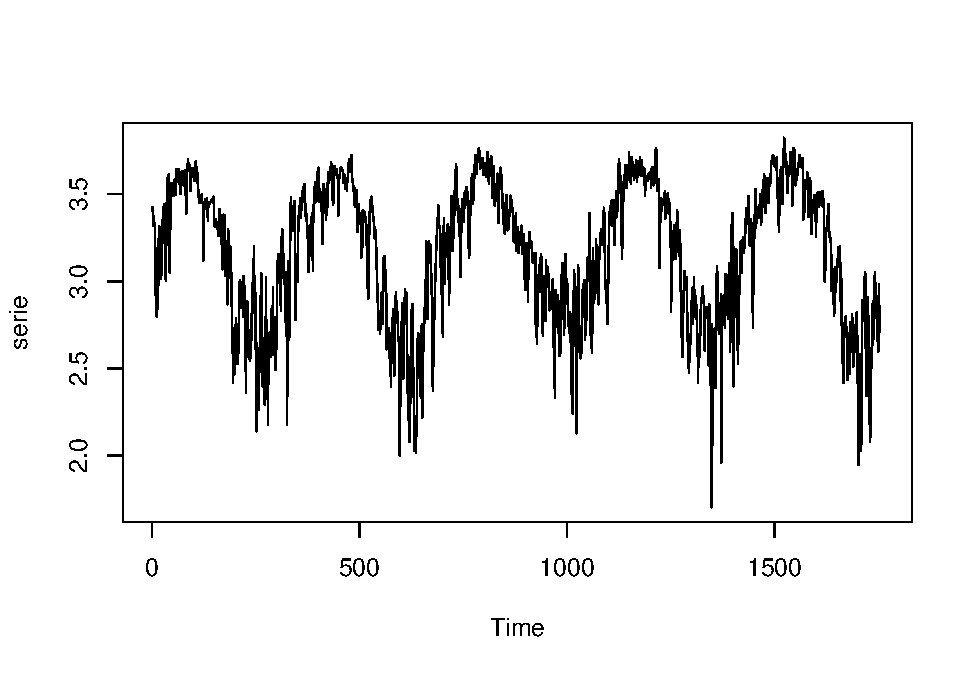
\includegraphics{timeSeries_files/figure-latex/unnamed-chunk-44-1.pdf}

Modelamos la tendencia, la cual podemos aparentemente ajustarla de forma
lineal, sabiendo que:\\
serie = parametroA * tiempo + parametroB\\
Con ayuda de la función lm calculamos dichos parámetros:

\begin{Shaded}
\begin{Highlighting}[]
\NormalTok{parametros.H1 =}\StringTok{ }\KeywordTok{lm}\NormalTok{(serie }\OperatorTok{~}\NormalTok{tiempo) }
\NormalTok{parametros.H1}
\end{Highlighting}
\end{Shaded}

\begin{verbatim}
## 
## Call:
## lm(formula = serie ~ tiempo)
## 
## Coefficients:
## (Intercept)       tiempo  
##   3.209e+00   -4.589e-05
\end{verbatim}

Tomamos Intercept como termino independiente (parametroB) y el otro como
el que multiplica al tiempo para poder calcular la serie (parametroA).
Para modelar la tendencia usamos la fórmula descrita antes:

\begin{Shaded}
\begin{Highlighting}[]
\CommentTok{# tendencia estimada para los datos de train }
\NormalTok{tendEstimadaTr =}\StringTok{ }\NormalTok{parametros.H1}\OperatorTok{$}\NormalTok{coefficients[}\DecValTok{1}\NormalTok{] }\OperatorTok{+}\StringTok{ }\NormalTok{tiempo}\OperatorTok{*}\NormalTok{parametros.H1}\OperatorTok{$}\NormalTok{coefficients[}\DecValTok{2}\NormalTok{] }
\CommentTok{# tendencia estimada para las predicciones de test }
\NormalTok{tendEstimadaTs =}\StringTok{ }\NormalTok{parametros.H1}\OperatorTok{$}\NormalTok{coefficients[}\DecValTok{1}\NormalTok{] }\OperatorTok{+}\StringTok{ }\NormalTok{tiempoTs}\OperatorTok{*}\NormalTok{parametros.H1}\OperatorTok{$}\NormalTok{coefficients[}\DecValTok{2}\NormalTok{] }
\end{Highlighting}
\end{Shaded}

Comprobamos visualmente si la tendencia se ajusta al modelo que tenemos
de la serie temporal:

\begin{Shaded}
\begin{Highlighting}[]
\KeywordTok{plot.ts}\NormalTok{(serie, }\DataTypeTok{xlim=}\KeywordTok{c}\NormalTok{(}\DecValTok{1}\NormalTok{, tiempoTs[}\KeywordTok{length}\NormalTok{(tiempoTs)])) }
\KeywordTok{lines}\NormalTok{(tiempo, tendEstimadaTr, }\DataTypeTok{col =} \StringTok{"blue"}\NormalTok{) }
\KeywordTok{lines}\NormalTok{(tiempoTs, tendEstimadaTs, }\DataTypeTok{col =} \StringTok{"green"}\NormalTok{)}
\end{Highlighting}
\end{Shaded}

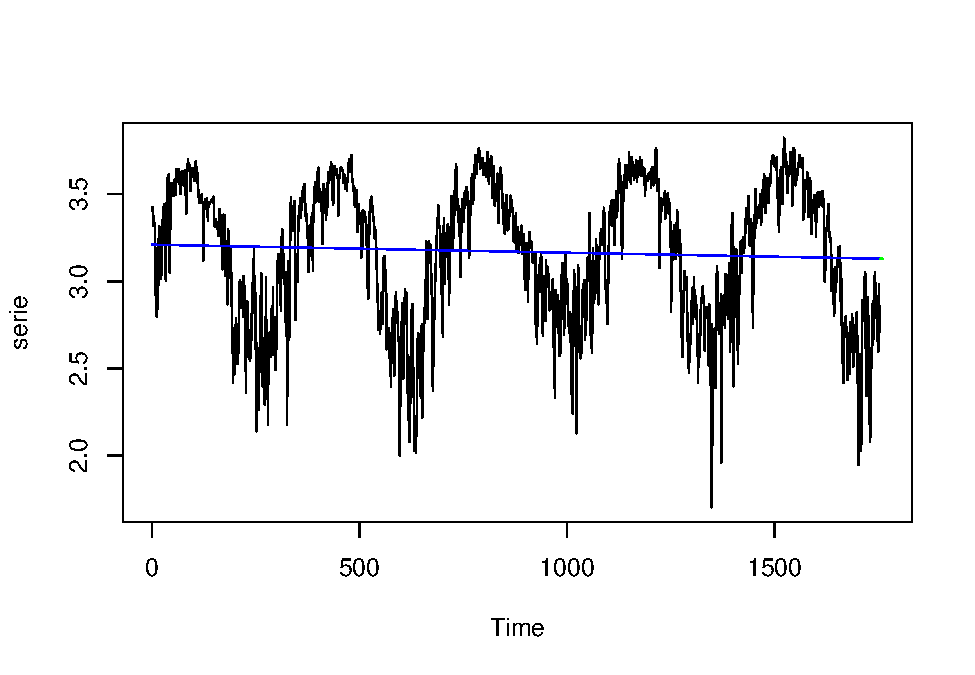
\includegraphics{timeSeries_files/figure-latex/unnamed-chunk-47-1.pdf}

Podemos observar los ajustes tanto de la tendencia para los datos de
train como de la estimada para los datos de test.

A continuación procedemos a validar de forma estadística que el modelo
lineal creado sea correcto. Con el test de Jarque Bera comprobamos si
los errores siguen una distribución normal a lo largo del tiempo.

\begin{Shaded}
\begin{Highlighting}[]
\NormalTok{JB =}\StringTok{ }\KeywordTok{jarque.bera.test}\NormalTok{(parametros.H1}\OperatorTok{$}\NormalTok{residuals)}
\NormalTok{JB}
\end{Highlighting}
\end{Shaded}

\begin{verbatim}
## 
##  Jarque Bera Test
## 
## data:  parametros.H1$residuals
## X-squared = 102.63, df = 2, p-value < 2.2e-16
\end{verbatim}

Como el valor del p-value es inferior a 0.05, no podemos asegurar que
los residuos no guarden una diferencia significativa con los datos de
una distribución normal, por lo que procedemos a intentar ajustar la
tendencia con otro modelo, esta vez cuadrático.

\begin{Shaded}
\begin{Highlighting}[]
\CommentTok{# calculo de parámetros}
\NormalTok{parametros.H1 =}\StringTok{ }\KeywordTok{lm}\NormalTok{(serie }\OperatorTok{~}\NormalTok{tiempo }\OperatorTok{+}\StringTok{ }\KeywordTok{I}\NormalTok{(tiempo}\OperatorTok{^}\DecValTok{2}\NormalTok{)) }
\NormalTok{parametros.H1}
\end{Highlighting}
\end{Shaded}

\begin{verbatim}
## 
## Call:
## lm(formula = serie ~ tiempo + I(tiempo^2))
## 
## Coefficients:
## (Intercept)       tiempo  I(tiempo^2)  
##   3.199e+00   -9.575e-06   -2.069e-08
\end{verbatim}

\begin{Shaded}
\begin{Highlighting}[]
\CommentTok{# tendencia estimada para los datos de train }
\NormalTok{tendEstimadaTr =}\StringTok{ }\NormalTok{parametros.H1}\OperatorTok{$}\NormalTok{coefficients[}\DecValTok{1}\NormalTok{] }\OperatorTok{+}\StringTok{ }\NormalTok{tiempo}\OperatorTok{*}\NormalTok{parametros.H1}\OperatorTok{$}\NormalTok{coefficients[}\DecValTok{2}\NormalTok{]  }\OperatorTok{+}\StringTok{ }\NormalTok{tiempo}\OperatorTok{*}\NormalTok{parametros.H1}\OperatorTok{$}\NormalTok{coefficients[}\DecValTok{3}\NormalTok{] }
\CommentTok{# tendencia estimada para las predicciones de test }
\NormalTok{tendEstimadaTs =}\StringTok{ }\NormalTok{parametros.H1}\OperatorTok{$}\NormalTok{coefficients[}\DecValTok{1}\NormalTok{] }\OperatorTok{+}\StringTok{ }\NormalTok{tiempoTs}\OperatorTok{*}\NormalTok{parametros.H1}\OperatorTok{$}\NormalTok{coefficients[}\DecValTok{2}\NormalTok{]  }\OperatorTok{+}\StringTok{ }\NormalTok{tiempoTs}\OperatorTok{*}\NormalTok{parametros.H1}\OperatorTok{$}\NormalTok{coefficients[}\DecValTok{3}\NormalTok{] }
\end{Highlighting}
\end{Shaded}

Comprobamos visualmente si la tendencia se ajusta al modelo que tenemos
de la serie temporal:

\begin{Shaded}
\begin{Highlighting}[]
\KeywordTok{plot.ts}\NormalTok{(serie, }\DataTypeTok{xlim=}\KeywordTok{c}\NormalTok{(}\DecValTok{1}\NormalTok{, tiempoTs[}\KeywordTok{length}\NormalTok{(tiempoTs)])) }
\KeywordTok{lines}\NormalTok{(tiempo, tendEstimadaTr, }\DataTypeTok{col =} \StringTok{"blue"}\NormalTok{) }
\KeywordTok{lines}\NormalTok{(tiempoTs, tendEstimadaTs, }\DataTypeTok{col =} \StringTok{"green"}\NormalTok{)}
\end{Highlighting}
\end{Shaded}

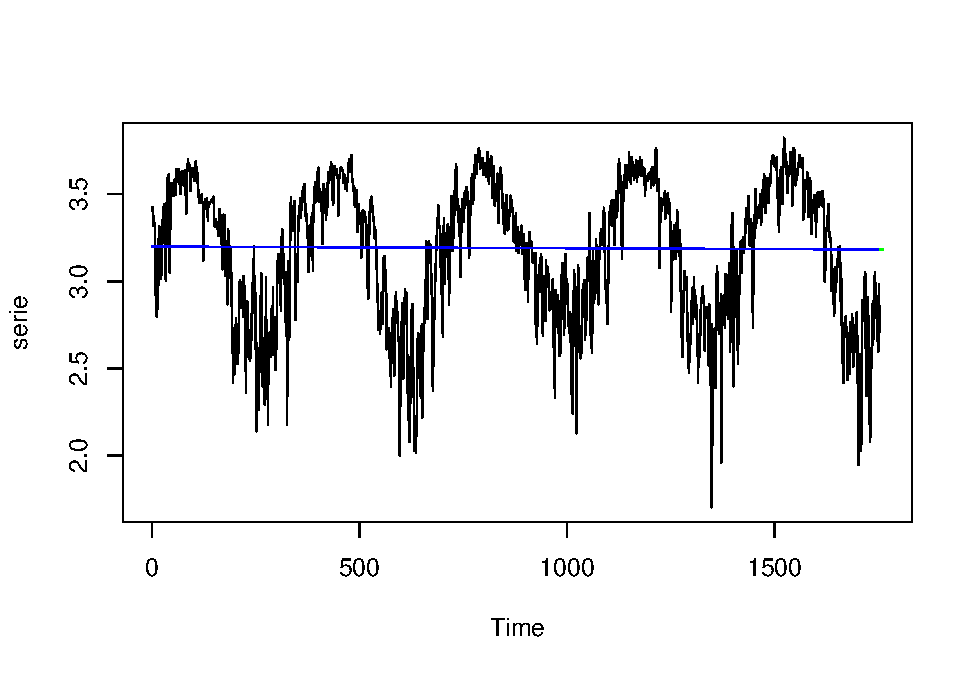
\includegraphics{timeSeries_files/figure-latex/unnamed-chunk-50-1.pdf}

Validamos de forma estadística de nuevo con el test de Jarque Bera, con
el que comprobamos si los errores siguen una distribución normal a lo
largo del tiempo.

\begin{Shaded}
\begin{Highlighting}[]
\NormalTok{JB =}\StringTok{ }\KeywordTok{jarque.bera.test}\NormalTok{(parametros.H1}\OperatorTok{$}\NormalTok{residuals)}
\NormalTok{JB}
\end{Highlighting}
\end{Shaded}

\begin{verbatim}
## 
##  Jarque Bera Test
## 
## data:  parametros.H1$residuals
## X-squared = 102.26, df = 2, p-value < 2.2e-16
\end{verbatim}

Una vez más, no logramos modelar la tendencia de manera correcta, veamos
como se comporta con una transformación logarítmica:

\begin{Shaded}
\begin{Highlighting}[]
\CommentTok{# calculo de parametros}
\NormalTok{parametros.H1 =}\StringTok{ }\KeywordTok{lm}\NormalTok{(serie }\OperatorTok{~}\StringTok{ }\KeywordTok{log}\NormalTok{(tiempo))}

\CommentTok{# tendencia estimada para los datos de train }
\NormalTok{tendEstimadaTr =}\StringTok{ }\NormalTok{parametros.H1}\OperatorTok{$}\NormalTok{coefficients[}\DecValTok{1}\NormalTok{] }\OperatorTok{+}\StringTok{ }\NormalTok{tiempo}\OperatorTok{*}\NormalTok{parametros.H1}\OperatorTok{$}\NormalTok{coefficients[}\DecValTok{2}\NormalTok{] }
\CommentTok{# tendencia estimada para las predicciones de test }
\NormalTok{tendEstimadaTs =}\StringTok{ }\NormalTok{parametros.H1}\OperatorTok{$}\NormalTok{coefficients[}\DecValTok{1}\NormalTok{] }\OperatorTok{+}\StringTok{ }\NormalTok{tiempoTs}\OperatorTok{*}\NormalTok{parametros.H1}\OperatorTok{$}\NormalTok{coefficients[}\DecValTok{2}\NormalTok{] }

\CommentTok{# representacion de la tendencia sobre la serie}
\KeywordTok{plot.ts}\NormalTok{(serie, }\DataTypeTok{xlim=}\KeywordTok{c}\NormalTok{(}\DecValTok{1}\NormalTok{, tiempoTs[}\KeywordTok{length}\NormalTok{(tiempoTs)])) }
\KeywordTok{lines}\NormalTok{(tiempo, tendEstimadaTr, }\DataTypeTok{col =} \StringTok{"blue"}\NormalTok{) }
\KeywordTok{lines}\NormalTok{(tiempoTs, tendEstimadaTs, }\DataTypeTok{col =} \StringTok{"green"}\NormalTok{)}
\end{Highlighting}
\end{Shaded}

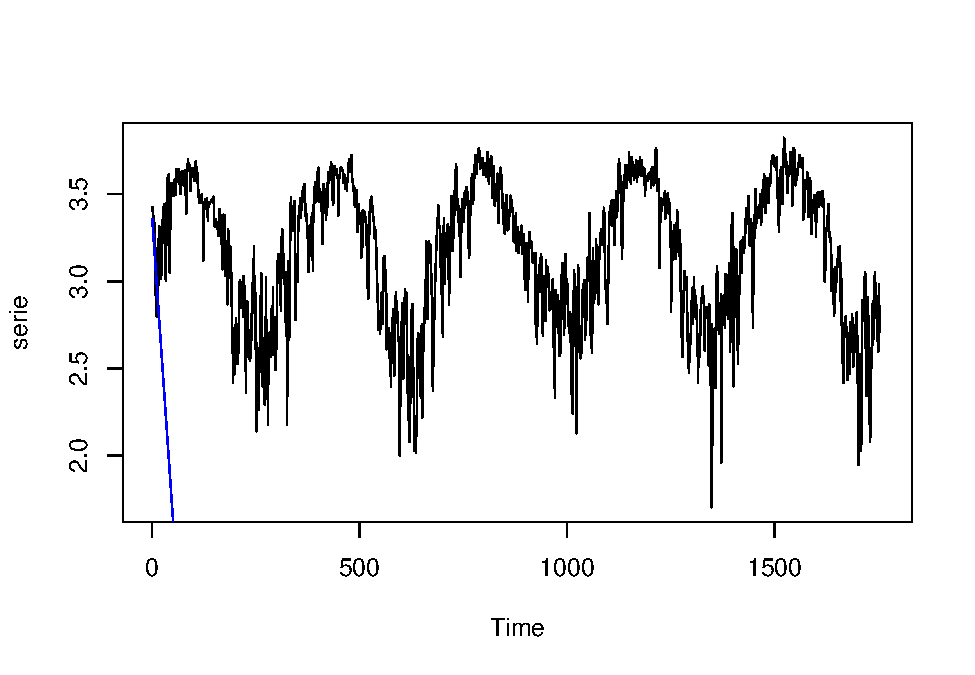
\includegraphics{timeSeries_files/figure-latex/unnamed-chunk-52-1.pdf}

\begin{Shaded}
\begin{Highlighting}[]
\CommentTok{# test de normalizacion Jarque Bera}
\NormalTok{JB =}\StringTok{ }\KeywordTok{jarque.bera.test}\NormalTok{(parametros.H1}\OperatorTok{$}\NormalTok{residuals)}
\NormalTok{JB}
\end{Highlighting}
\end{Shaded}

\begin{verbatim}
## 
##  Jarque Bera Test
## 
## data:  parametros.H1$residuals
## X-squared = 99.71, df = 2, p-value < 2.2e-16
\end{verbatim}

Como última prueba de transformaciones matemáticas aplicadas para
modelar la tendencia de la serie, procedo a intentarlo con una
sinusoidal:

\begin{Shaded}
\begin{Highlighting}[]
\CommentTok{# calculo de parametros}
\NormalTok{parametros.H1 =}\StringTok{ }\KeywordTok{lm}\NormalTok{(serie }\OperatorTok{~}\StringTok{ }\KeywordTok{sin}\NormalTok{(tiempo))}

\CommentTok{# tendencia estimada para los datos de train }
\NormalTok{tendEstimadaTr =}\StringTok{ }\NormalTok{parametros.H1}\OperatorTok{$}\NormalTok{coefficients[}\DecValTok{1}\NormalTok{] }\OperatorTok{+}\StringTok{ }\NormalTok{tiempo}\OperatorTok{*}\NormalTok{parametros.H1}\OperatorTok{$}\NormalTok{coefficients[}\DecValTok{2}\NormalTok{] }
\CommentTok{# tendencia estimada para las predicciones de test }
\NormalTok{tendEstimadaTs =}\StringTok{ }\NormalTok{parametros.H1}\OperatorTok{$}\NormalTok{coefficients[}\DecValTok{1}\NormalTok{] }\OperatorTok{+}\StringTok{ }\NormalTok{tiempoTs}\OperatorTok{*}\NormalTok{parametros.H1}\OperatorTok{$}\NormalTok{coefficients[}\DecValTok{2}\NormalTok{] }

\CommentTok{# representacion de la tendencia sobre la serie}
\KeywordTok{plot.ts}\NormalTok{(serie, }\DataTypeTok{xlim=}\KeywordTok{c}\NormalTok{(}\DecValTok{1}\NormalTok{, tiempoTs[}\KeywordTok{length}\NormalTok{(tiempoTs)])) }
\KeywordTok{lines}\NormalTok{(tiempo, tendEstimadaTr, }\DataTypeTok{col =} \StringTok{"blue"}\NormalTok{) }
\KeywordTok{lines}\NormalTok{(tiempoTs, tendEstimadaTs, }\DataTypeTok{col =} \StringTok{"green"}\NormalTok{)}
\end{Highlighting}
\end{Shaded}

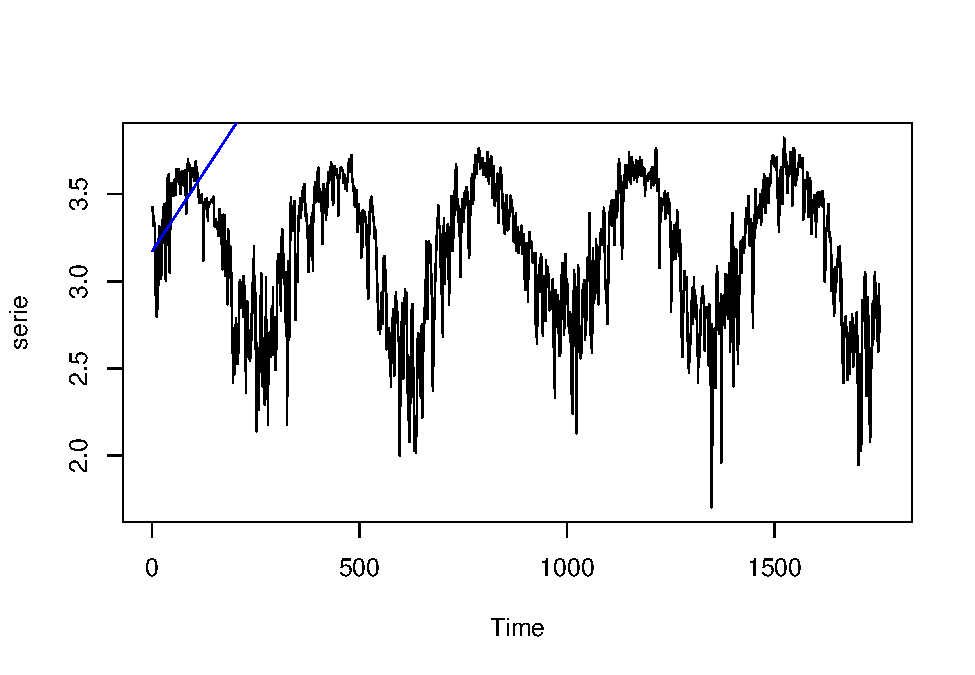
\includegraphics{timeSeries_files/figure-latex/unnamed-chunk-53-1.pdf}

\begin{Shaded}
\begin{Highlighting}[]
\CommentTok{# test de normalizacion Jarque Bera}
\NormalTok{JB =}\StringTok{ }\KeywordTok{jarque.bera.test}\NormalTok{(parametros.H1}\OperatorTok{$}\NormalTok{residuals)}
\NormalTok{JB}
\end{Highlighting}
\end{Shaded}

\begin{verbatim}
## 
##  Jarque Bera Test
## 
## data:  parametros.H1$residuals
## X-squared = 106.92, df = 2, p-value < 2.2e-16
\end{verbatim}

Tras probar con estos distintos modelos obtenidos mediante diferentes
transformaciones matemáticas, me decido por realizar diferenciación
tantas veces como sea necesario con tal de suazivar la tendencia:

Probamos de nuevo\ldots{}

\begin{Shaded}
\begin{Highlighting}[]
\NormalTok{serie2=}\KeywordTok{diff}\NormalTok{(serie, }\DataTypeTok{differences =} \DecValTok{3}\NormalTok{)}
\NormalTok{tiempo2=}\StringTok{ }\DecValTok{1}\OperatorTok{:}\KeywordTok{length}\NormalTok{(serie2)}
\CommentTok{# calculo de parametros}
\NormalTok{parametros.H1 =}\StringTok{ }\KeywordTok{lm}\NormalTok{(serie2 }\OperatorTok{~}\StringTok{ }\NormalTok{tiempo2)}

\CommentTok{# tendencia estimada para los datos de train }
\NormalTok{tendEstimadaTr =}\StringTok{ }\NormalTok{parametros.H1}\OperatorTok{$}\NormalTok{coefficients[}\DecValTok{1}\NormalTok{] }\OperatorTok{+}\StringTok{ }\NormalTok{tiempo2}\OperatorTok{*}\NormalTok{parametros.H1}\OperatorTok{$}\NormalTok{coefficients[}\DecValTok{2}\NormalTok{] }
\CommentTok{# tendencia estimada para las predicciones de test }
\NormalTok{tendEstimadaTs =}\StringTok{ }\NormalTok{parametros.H1}\OperatorTok{$}\NormalTok{coefficients[}\DecValTok{1}\NormalTok{] }\OperatorTok{+}\StringTok{ }\NormalTok{tiempoTs}\OperatorTok{*}\NormalTok{parametros.H1}\OperatorTok{$}\NormalTok{coefficients[}\DecValTok{2}\NormalTok{] }

\CommentTok{# representacion de la tendencia sobre la serie}
\KeywordTok{plot.ts}\NormalTok{(serie2, }\DataTypeTok{xlim=}\KeywordTok{c}\NormalTok{(}\DecValTok{1}\NormalTok{, tiempoTs[}\KeywordTok{length}\NormalTok{(tiempoTs)])) }
\KeywordTok{lines}\NormalTok{(tiempo2, tendEstimadaTr, }\DataTypeTok{col =} \StringTok{"blue"}\NormalTok{) }
\KeywordTok{lines}\NormalTok{(tiempoTs, tendEstimadaTs, }\DataTypeTok{col =} \StringTok{"green"}\NormalTok{)}
\end{Highlighting}
\end{Shaded}

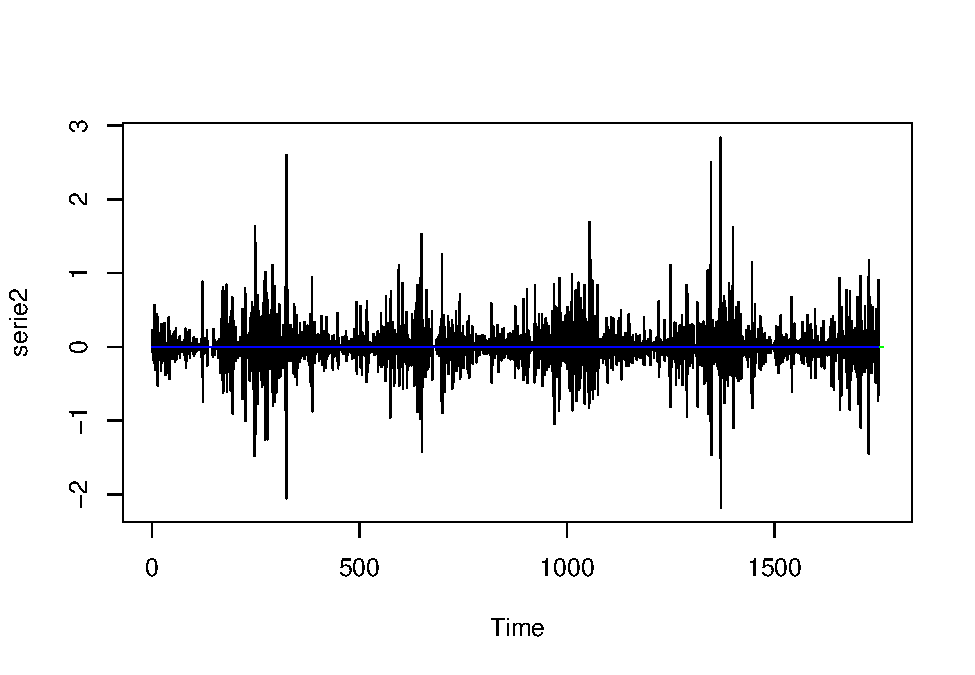
\includegraphics{timeSeries_files/figure-latex/unnamed-chunk-54-1.pdf}

\begin{Shaded}
\begin{Highlighting}[]
\CommentTok{# test de normalizacion Jarque Bera}
\NormalTok{JB =}\StringTok{ }\KeywordTok{jarque.bera.test}\NormalTok{(parametros.H1}\OperatorTok{$}\NormalTok{residuals)}
\NormalTok{JB}
\end{Highlighting}
\end{Shaded}

\begin{verbatim}
## 
##  Jarque Bera Test
## 
## data:  parametros.H1$residuals
## X-squared = 7374.5, df = 2, p-value < 2.2e-16
\end{verbatim}

Como podemos observar, tras las pruebas de modelado de tendencia tanto
con diversas transformaciones matemáticas (logarítmica, cuadrática,
senoidal) como por diferenciación de la serie con el fin de suavizar la
tendencia, no logramos que los residuos de las diversas tendencias
calculadas pasen el test de Jarque Bera, por lo que es posible con alta
probabilidad que dichos residuos no sigan una distribución normal.
Conociendo este dato, es posible que no haya conseguido modelar la
tendencia con ninguno de los modelos obtenidos, por tanto me decido por
no restársela a la serie en los siguientes pasos de este ejercicio.

Tras este extenso estudio de la tendencia, procedemos a hayar y eliminar
la estacionalidad de la seria:

\begin{Shaded}
\begin{Highlighting}[]
\NormalTok{k =}\StringTok{ }\DecValTok{365} \CommentTok{# aquí guardamos los datos estacionales }
\NormalTok{estacionalidad =}\StringTok{ }\KeywordTok{decompose}\NormalTok{(serie.ts.log)}\OperatorTok{$}\NormalTok{seasonal[}\DecValTok{1}\OperatorTok{:}\NormalTok{k]}
\CommentTok{# elminamos la estacionalidad}
\NormalTok{serie.sinEst =}\StringTok{ }\NormalTok{serie }\OperatorTok{-}\StringTok{ }\NormalTok{estacionalidad}
\end{Highlighting}
\end{Shaded}

\begin{verbatim}
## Warning in serie - estacionalidad: longitud de objeto mayor no es múltiplo
## de la longitud de uno menor
\end{verbatim}

Comprobamos como se queda la serie sin dicha estacionalidad

\begin{Shaded}
\begin{Highlighting}[]
\KeywordTok{plot.ts}\NormalTok{(serie.sinEst, }\DataTypeTok{xlim=}\KeywordTok{c}\NormalTok{(}\DecValTok{1}\NormalTok{, tiempoTs[}\KeywordTok{length}\NormalTok{(tiempoTs)]))}
\end{Highlighting}
\end{Shaded}

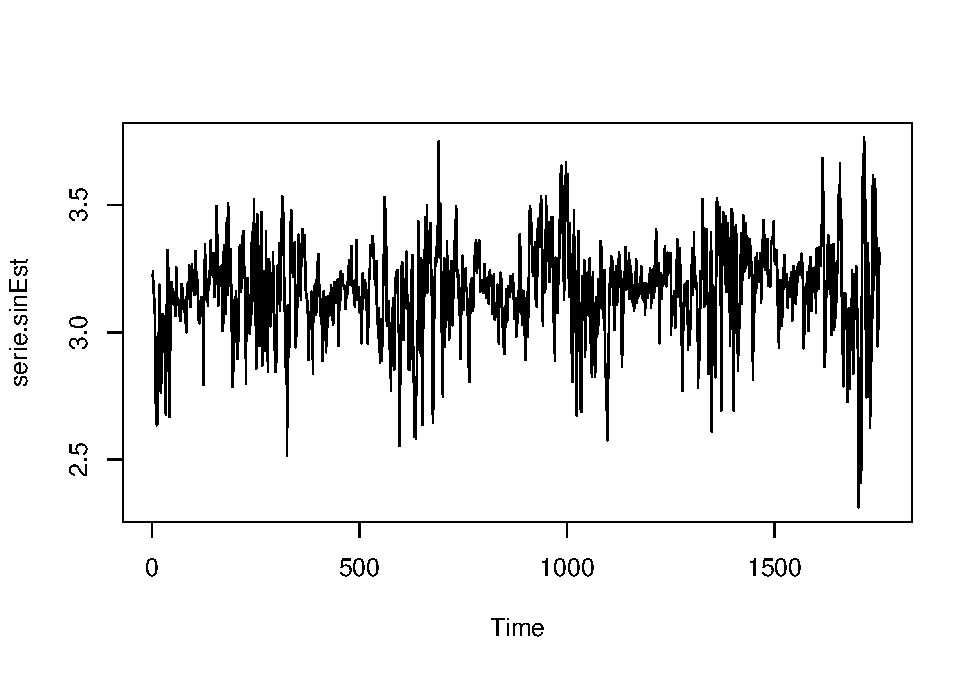
\includegraphics{timeSeries_files/figure-latex/unnamed-chunk-56-1.pdf}

Ahora que tan solo nos queda la componente irregular tras haber
eliminado la componente de estacionalidad, procedemos a comprobar si la
serie es estacionaria o no mediante el test ACF.

\begin{Shaded}
\begin{Highlighting}[]
\KeywordTok{acf}\NormalTok{(serie.sinEst)}
\end{Highlighting}
\end{Shaded}

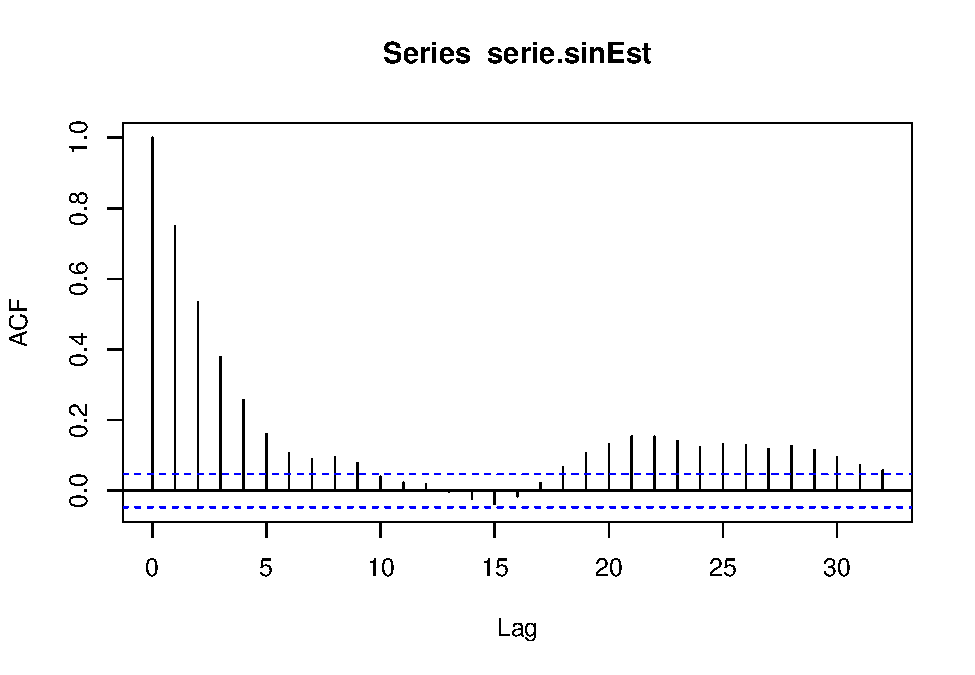
\includegraphics{timeSeries_files/figure-latex/unnamed-chunk-57-1.pdf}

Observando este gráfico acf, puede caber la posibilidad de tomar como
`'bajada lenta'' de los datos con respecto a los instantes sucesivos de
tiempo, para asegurarnos de la estacionariedad de la serie, procedemos a
realizar el test de Dickey-Fuller aumentado:

\begin{Shaded}
\begin{Highlighting}[]
\KeywordTok{adf.test}\NormalTok{(serie.sinEst)}
\end{Highlighting}
\end{Shaded}

\begin{verbatim}
## Warning in adf.test(serie.sinEst): p-value smaller than printed p-value
\end{verbatim}

\begin{verbatim}
## 
##  Augmented Dickey-Fuller Test
## 
## data:  serie.sinEst
## Dickey-Fuller = -10.378, Lag order = 12, p-value = 0.01
## alternative hypothesis: stationary
\end{verbatim}

Al tomar como hipótesis nula que la serie es estacionaria y al ser el
p-value inferior a 0.05, podemos asegurar con un 95\% de probabilidad
que la serie es estacionaria, por tanto la tomamos así. Debido a esto no
será necesario realizar diferenciación para convertir la serie en
estacionaria.

Observamos el acf parcial para ver como influyen de forma individual
cada uno de los instantes de tiempo sobre el instante actual.

\begin{Shaded}
\begin{Highlighting}[]
\KeywordTok{pacf}\NormalTok{(serie.sinEst)}
\end{Highlighting}
\end{Shaded}

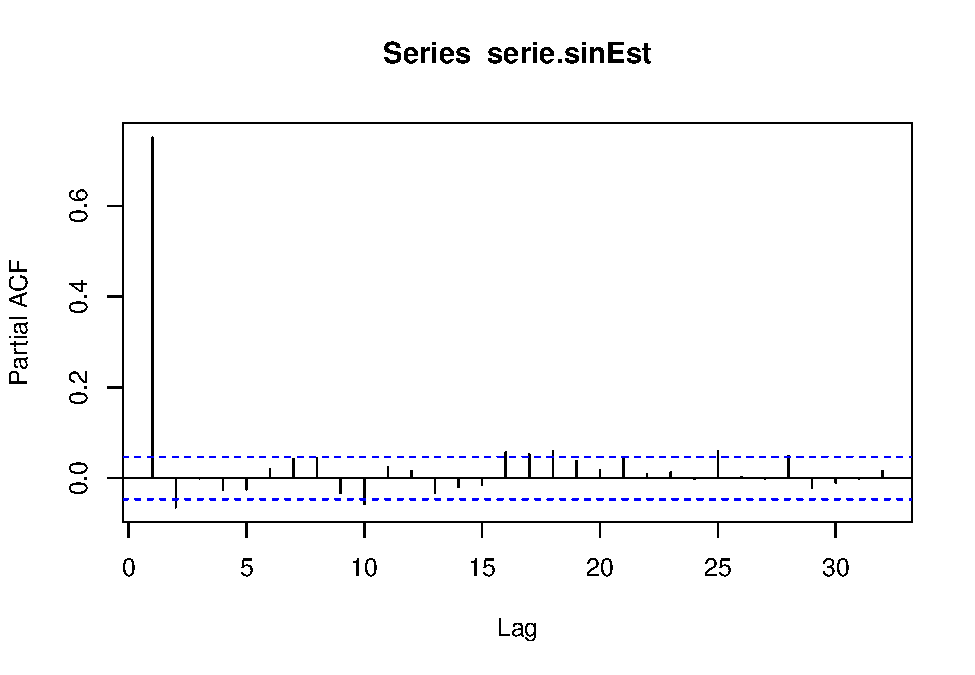
\includegraphics{timeSeries_files/figure-latex/unnamed-chunk-59-1.pdf}

Observando los gráficos ofrecidos por acf y pacf, y sabiendo que la
serie es estacionaria gracias al test de Dickey-Fuller, me resulta
coherente pensar en un modelo de medias móviles de grado 22 para modelar
la serie temporal mediante ARIMA. La elección del modelo es debido a que
en pacf existe una bajada en los datos drástica y una estabilización en
forma de `'olas'', escogiendo el grado del modelo con ayuda del ultimo
de los datos que traspasan de forma clara el umbral mínimo en el gráfico
acf. Entrenamos el modelo escogido a continuación:

\begin{Shaded}
\begin{Highlighting}[]
\CommentTok{# coeficiente de autoregresión = 0, diferenciaciones = 0, coeficiente de medias moviles = 0 }
\NormalTok{modelo =}\StringTok{ }\KeywordTok{arima}\NormalTok{(serie.sinEst, }\DataTypeTok{order =} \KeywordTok{c}\NormalTok{(}\DecValTok{0}\NormalTok{,}\DecValTok{0}\NormalTok{,}\DecValTok{22}\NormalTok{))}
\CommentTok{# calculamos las predicciones }
\NormalTok{predicciones =}\StringTok{ }\KeywordTok{predict}\NormalTok{(modelo, }\DataTypeTok{n.ahead =}\NormalTok{ Npred) }
\NormalTok{valoresPredichos =}\StringTok{ }\NormalTok{predicciones}\OperatorTok{$}\NormalTok{pred }
\NormalTok{valoresPredichos}
\end{Highlighting}
\end{Shaded}

\begin{verbatim}
## Time Series:
## Start = 1755 
## End = 1761 
## Frequency = 1 
## [1] 3.291288 3.209668 3.159646 3.177438 3.152966 3.171279 3.196229
\end{verbatim}

Observamos ahora de forma visual el modelo incluyendo la serie sin
estacionalidad:

\begin{Shaded}
\begin{Highlighting}[]
\KeywordTok{plot.ts}\NormalTok{(serie.sinEst, }\DataTypeTok{xlim=}\KeywordTok{c}\NormalTok{(}\DecValTok{1500}\NormalTok{, tiempoTs[}\KeywordTok{length}\NormalTok{(tiempoTs)])) }
\KeywordTok{lines}\NormalTok{(tiempoTs,valoresPredichos, }\DataTypeTok{col=}\StringTok{"green"}\NormalTok{)}
\end{Highlighting}
\end{Shaded}

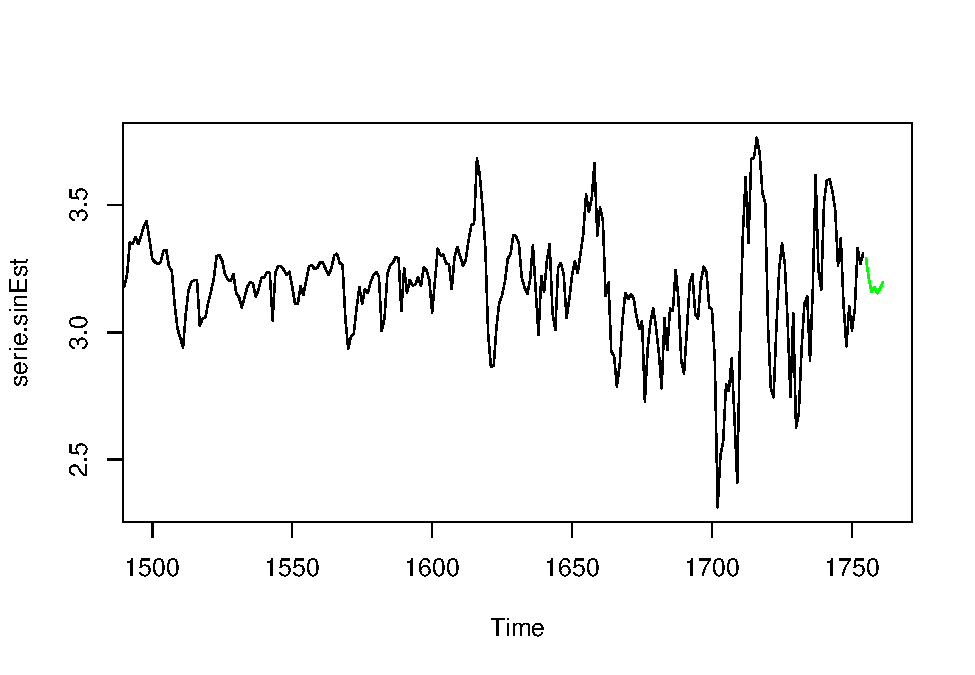
\includegraphics{timeSeries_files/figure-latex/unnamed-chunk-61-1.pdf}

Parece ser que las predicciones obtenidas hasta el momento caen dentro
de los límites razonables de la serie.

Finalmente probamos la validez de nuestro modelo (sus errores) mediante
tests estadísticos.\\
Aplicamos varios:

Test de Box-Pierce: comprobamos que los residuos que nos quedan son
aleatorios:

\begin{Shaded}
\begin{Highlighting}[]
\KeywordTok{Box.test}\NormalTok{(modelo}\OperatorTok{$}\NormalTok{residuals)}
\end{Highlighting}
\end{Shaded}

\begin{verbatim}
## 
##  Box-Pierce test
## 
## data:  modelo$residuals
## X-squared = 0.003811, df = 1, p-value = 0.9508
\end{verbatim}

Este valor de p-value nos dice con un 95\% de confianza que los errores
obtenidos por el modelo creado son aleatorios, por lo que el modelo
queda validado por este test. Continuamos con los tests de normalidad.

Jarque Bera: vemos si los residuos, aunque aleatorios, son normales
(media cero y desviación típica la que sea).

\begin{Shaded}
\begin{Highlighting}[]
\KeywordTok{jarque.bera.test}\NormalTok{(modelo}\OperatorTok{$}\NormalTok{residuals)}
\end{Highlighting}
\end{Shaded}

\begin{verbatim}
## 
##  Jarque Bera Test
## 
## data:  modelo$residuals
## X-squared = 910.17, df = 2, p-value < 2.2e-16
\end{verbatim}

Saphiro-Wilk: mismo cometido que Jarque Bera

\begin{Shaded}
\begin{Highlighting}[]
\KeywordTok{shapiro.test}\NormalTok{(modelo}\OperatorTok{$}\NormalTok{residuals)}
\end{Highlighting}
\end{Shaded}

\begin{verbatim}
## 
##  Shapiro-Wilk normality test
## 
## data:  modelo$residuals
## W = 0.95311, p-value < 2.2e-16
\end{verbatim}

Asumimos, con alta probabilidad, tras la ejecución de ambos tests que
los residuos no siguen una distribución normal debido a los p-values
obtenidos, ya que la hipótesis nula propone que los datos no siguen una
distribución normal. A continuación obtenemos un histograma y función de
densidad para obtener resultados gráficos de confirmación.

\begin{Shaded}
\begin{Highlighting}[]
\KeywordTok{hist}\NormalTok{(modelo}\OperatorTok{$}\NormalTok{residuals, }\DataTypeTok{col=}\StringTok{"blue"}\NormalTok{, }\DataTypeTok{prob=}\NormalTok{T,}\DataTypeTok{ylim=}\KeywordTok{c}\NormalTok{(}\DecValTok{0}\NormalTok{,}\DecValTok{6}\NormalTok{), }\DataTypeTok{xlim=}\KeywordTok{c}\NormalTok{(}\OperatorTok{-}\FloatTok{0.4}\NormalTok{,}\FloatTok{0.4}\NormalTok{)) }
\KeywordTok{lines}\NormalTok{(}\KeywordTok{density}\NormalTok{(modelo}\OperatorTok{$}\NormalTok{residuals))}
\end{Highlighting}
\end{Shaded}

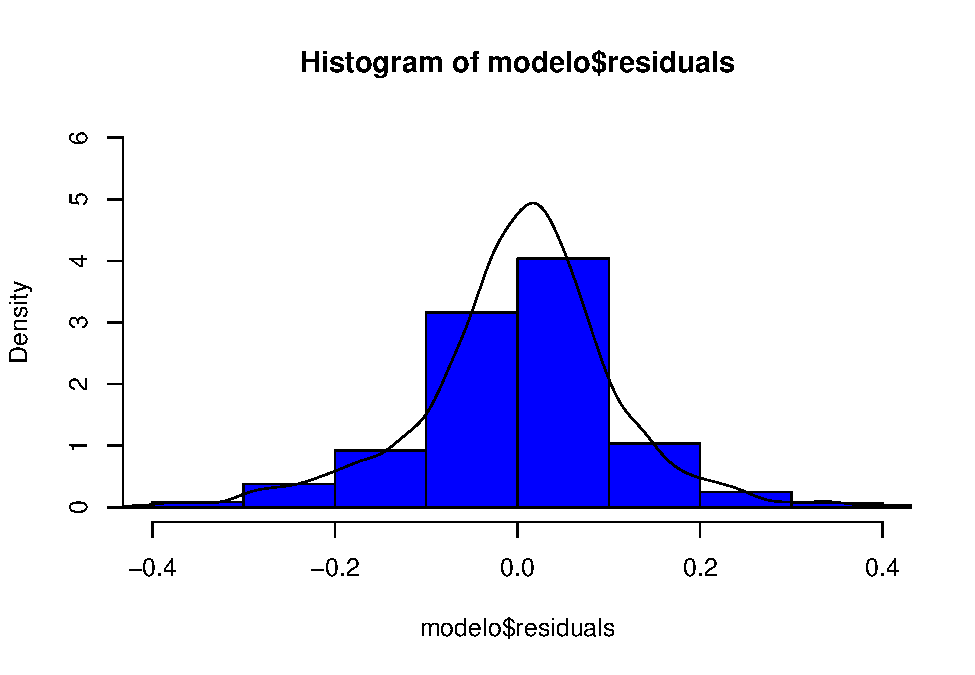
\includegraphics{timeSeries_files/figure-latex/unnamed-chunk-65-1.pdf}

Como podemos observar, el histograma representando la distribución de
los residuos del modelo nos dice que estos sí que siguen una
distribución normal, al contrario que los tests de Sphiro-Wilk y Jarque
Bera. Llegados a este punto, nos acogeremos a la validez del teorema del
límite central para asumir que, teniendo la cantidad elevada de datos
que tenemos, los cuales toman una varianza no nula pero finita, estos se
ajustan de buena forma a los de una distribución normal, dando por
válida la representación de la distribución de los residuos dados por el
histograma y por tanto, el modelo obtenido.

Con estas comprobaciones el modelo queda validado, ya que los errores
que nos dan son aleatorios que provienen de una distribución normal. A
continuación hemos de deshacer los cambios para obtener los predicciones
reales:

\begin{Shaded}
\begin{Highlighting}[]
\CommentTok{# obtenemos la estacionalidad correspondiente restandole a los dias del año al completo (365)}
\CommentTok{# la cantidad de dias que hay entre el mes de inicio del dataset (7 de mayo) y el comienzo del}
\CommentTok{# día y el mes que queremos predecir (1 de marzo)}
\NormalTok{estacionalidadCorrespondiente =}\StringTok{ }\DecValTok{365}\OperatorTok{-}\DecValTok{30}\OperatorTok{-}\DecValTok{31}\OperatorTok{-}\DecValTok{7}

\CommentTok{# incluimos la estacionalidad}
\NormalTok{valoresPredichos.Est =}\StringTok{ }
\StringTok{  }\NormalTok{valoresPredichos }\OperatorTok{+}\StringTok{ }\NormalTok{estacionalidad[estacionalidadCorrespondiente }\OperatorTok{:}\StringTok{ }\NormalTok{(estacionalidadCorrespondiente}\OperatorTok{+}\DecValTok{6}\NormalTok{)]}

\CommentTok{# Transformación de los logaritmos}
\NormalTok{valoresPredichos.Est.exp =}\StringTok{ }\KeywordTok{exp}\NormalTok{(valoresPredichos.Est)}

\CommentTok{# usamos exp(serie) por haber hecho al principio serie = log(serie) }
\KeywordTok{plot.ts}\NormalTok{(}\KeywordTok{exp}\NormalTok{(serie),}\DataTypeTok{xlim=}\KeywordTok{c}\NormalTok{(}\DecValTok{1500}\NormalTok{, tiempoTs[}\KeywordTok{length}\NormalTok{(tiempoTs)])) }
\KeywordTok{lines}\NormalTok{(tiempoTs, valoresPredichos.Est.exp, }\DataTypeTok{col =} \StringTok{"green"}\NormalTok{)}
\end{Highlighting}
\end{Shaded}

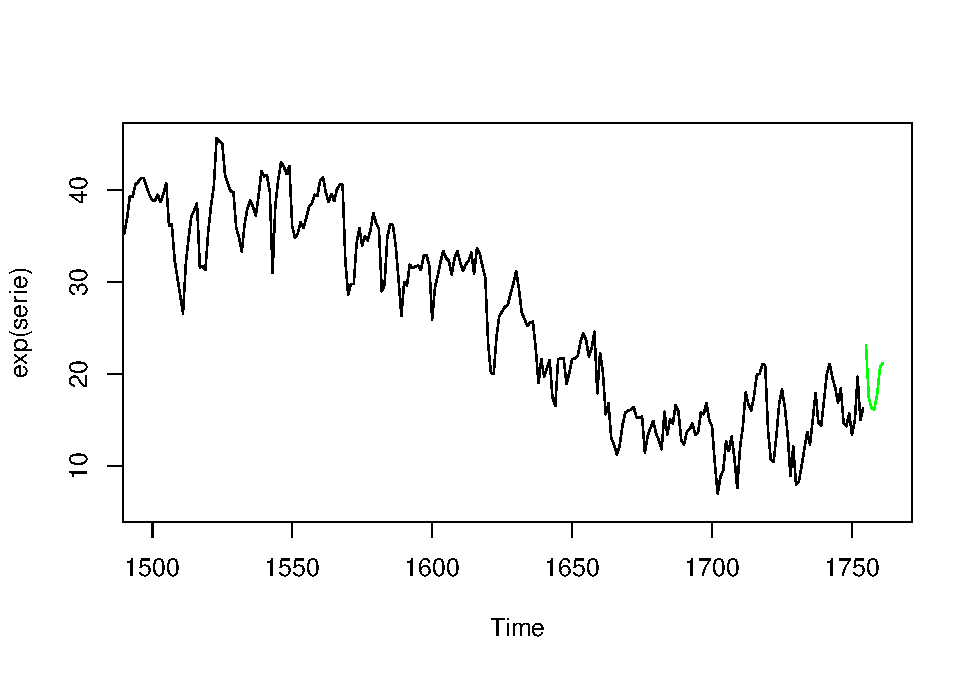
\includegraphics{timeSeries_files/figure-latex/unnamed-chunk-66-1.pdf}

Parecen razonables los resultados de predicción obtenidos, los cuales
son los siguientes para los 7 primeros días de Marzo de 2018:

\begin{Shaded}
\begin{Highlighting}[]
\NormalTok{valoresPredichos.Est.exp}
\end{Highlighting}
\end{Shaded}

\begin{verbatim}
## Time Series:
## Start = 1755 
## End = 1761 
## Frequency = 1 
## [1] 23.13305 17.42480 16.25250 16.13258 17.80971 20.71788 21.17717
\end{verbatim}


\end{document}
